\documentclass[1p]{elsarticle_modified}
%\bibliographystyle{elsarticle-num}

%\usepackage[colorlinks]{hyperref}
%\usepackage{abbrmath_seonhwa} %\Abb, \Ascr, \Acal ,\Abf, \Afrak
\usepackage{amsfonts}
\usepackage{amssymb}
\usepackage{amsmath}
\usepackage{amsthm}
\usepackage{scalefnt}
\usepackage{amsbsy}
\usepackage{kotex}
\usepackage{caption}
\usepackage{subfig}
\usepackage{color}
\usepackage{graphicx}
\usepackage{xcolor} %% white, black, red, green, blue, cyan, magenta, yellow
\usepackage{float}
\usepackage{setspace}
\usepackage{hyperref}

\usepackage{tikz}
\usetikzlibrary{arrows}

\usepackage{multirow}
\usepackage{array} % fixed length table
\usepackage{hhline}

%%%%%%%%%%%%%%%%%%%%%
\makeatletter
\renewcommand*\env@matrix[1][\arraystretch]{%
	\edef\arraystretch{#1}%
	\hskip -\arraycolsep
	\let\@ifnextchar\new@ifnextchar
	\array{*\c@MaxMatrixCols c}}
\makeatother %https://tex.stackexchange.com/questions/14071/how-can-i-increase-the-line-spacing-in-a-matrix
%%%%%%%%%%%%%%%

\usepackage[normalem]{ulem}

\newcommand{\msout}[1]{\ifmmode\text{\sout{\ensuremath{#1}}}\else\sout{#1}\fi}
%SOURCE: \msout is \stkout macro in https://tex.stackexchange.com/questions/20609/strikeout-in-math-mode

\newcommand{\cancel}[1]{
	\ifmmode
	{\color{red}\msout{#1}}
	\else
	{\color{red}\sout{#1}}
	\fi
}

\newcommand{\add}[1]{
	{\color{blue}\uwave{#1}}
}

\newcommand{\replace}[2]{
	\ifmmode
	{\color{red}\msout{#1}}{\color{blue}\uwave{#2}}
	\else
	{\color{red}\sout{#1}}{\color{blue}\uwave{#2}}
	\fi
}

\newcommand{\Sol}{\mathcal{S}} %segment
\newcommand{\D}{D} %diagram
\newcommand{\A}{\mathcal{A}} %arc


%%%%%%%%%%%%%%%%%%%%%%%%%%%%%5 test

\def\sl{\operatorname{\textup{SL}}(2,\Cbb)}
\def\psl{\operatorname{\textup{PSL}}(2,\Cbb)}
\def\quan{\mkern 1mu \triangleright \mkern 1mu}

\theoremstyle{definition}
\newtheorem{thm}{Theorem}[section]
\newtheorem{prop}[thm]{Proposition}
\newtheorem{lem}[thm]{Lemma}
\newtheorem{ques}[thm]{Question}
\newtheorem{cor}[thm]{Corollary}
\newtheorem{defn}[thm]{Definition}
\newtheorem{exam}[thm]{Example}
\newtheorem{rmk}[thm]{Remark}
\newtheorem{alg}[thm]{Algorithm}

\newcommand{\I}{\sqrt{-1}}
\begin{document}

%\begin{frontmatter}
%
%\title{Boundary parabolic representations of knots up to 8 crossings}
%
%%% Group authors per affiliation:
%\author{Yunhi Cho} 
%\address{Department of Mathematics, University of Seoul, Seoul, Korea}
%\ead{yhcho@uos.ac.kr}
%
%
%\author{Seonhwa Kim} %\fnref{s_kim}}
%\address{Center for Geometry and Physics, Institute for Basic Science, Pohang, 37673, Korea}
%\ead{ryeona17@ibs.re.kr}
%
%\author{Hyuk Kim}
%\address{Department of Mathematical Sciences, Seoul National University, Seoul 08826, Korea}
%\ead{hyukkim@snu.ac.kr}
%
%\author{Seokbeom Yoon}
%\address{Department of Mathematical Sciences, Seoul National University, Seoul, 08826,  Korea}
%\ead{sbyoon15@snu.ac.kr}
%
%\begin{abstract}
%We find all boundary parabolic representation of knots up to 8 crossings.
%
%\end{abstract}
%\begin{keyword}
%    \MSC[2010] 57M25 
%\end{keyword}
%
%\end{frontmatter}

%\linenumbers
%\tableofcontents
%
\newcommand\colored[1]{\textcolor{white}{\rule[-0.35ex]{0.8em}{1.4ex}}\kern-0.8em\color{red} #1}%
%\newcommand\colored[1]{\textcolor{white}{ #1}\kern-2.17ex	\textcolor{white}{ #1}\kern-1.81ex	\textcolor{white}{ #1}\kern-2.15ex\color{red}#1	}

{\Large $\underline{12a_{1187}~(K12a_{1187})}$}

\setlength{\tabcolsep}{10pt}
\renewcommand{\arraystretch}{1.6}
\vspace{1cm}\begin{tabular}{m{100pt}>{\centering\arraybackslash}m{274pt}}
\multirow{5}{120pt}{
	\centering
	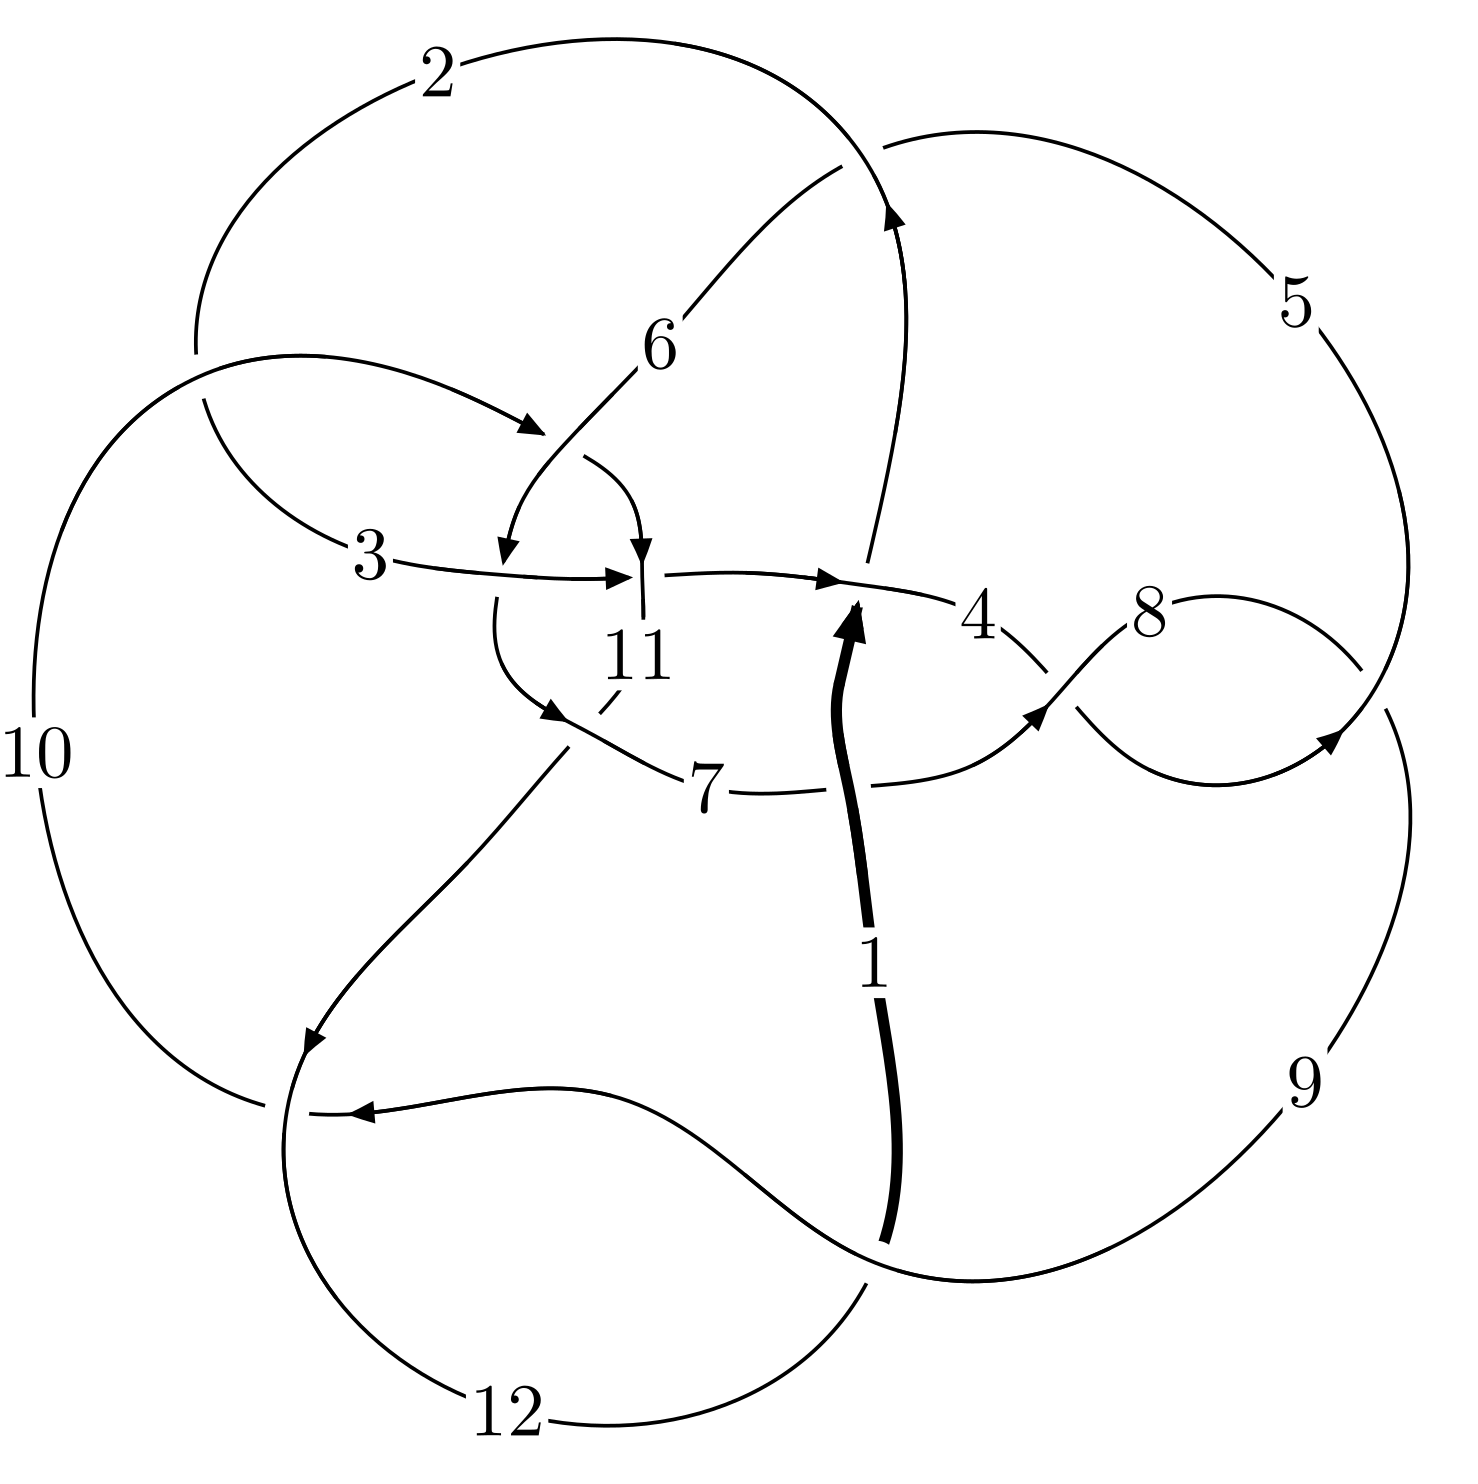
\includegraphics[width=112pt]{../../../GIT/diagram.site/Diagrams/png/1988_12a_1187.png}\\
\ \ \ A knot diagram\footnotemark}&
\allowdisplaybreaks
\textbf{Linearized knot diagam} \\
\cline{2-2}
 &
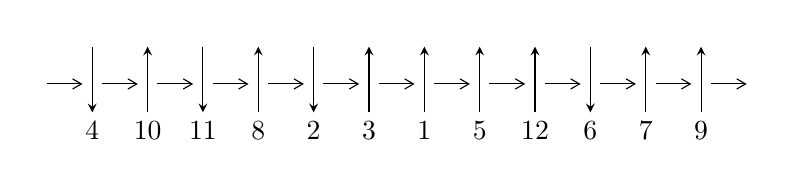
\begin{tikzpicture}[x=20pt, y=17pt]
	% nodes
	\node (C0) at (0, 0) {};
	\node (C1) at (1, 0) {};
	\node (C1U) at (1, +1) {};
	\node (C1D) at (1, -1) {4};

	\node (C2) at (2, 0) {};
	\node (C2U) at (2, +1) {};
	\node (C2D) at (2, -1) {10};

	\node (C3) at (3, 0) {};
	\node (C3U) at (3, +1) {};
	\node (C3D) at (3, -1) {11};

	\node (C4) at (4, 0) {};
	\node (C4U) at (4, +1) {};
	\node (C4D) at (4, -1) {8};

	\node (C5) at (5, 0) {};
	\node (C5U) at (5, +1) {};
	\node (C5D) at (5, -1) {2};

	\node (C6) at (6, 0) {};
	\node (C6U) at (6, +1) {};
	\node (C6D) at (6, -1) {3};

	\node (C7) at (7, 0) {};
	\node (C7U) at (7, +1) {};
	\node (C7D) at (7, -1) {1};

	\node (C8) at (8, 0) {};
	\node (C8U) at (8, +1) {};
	\node (C8D) at (8, -1) {5};

	\node (C9) at (9, 0) {};
	\node (C9U) at (9, +1) {};
	\node (C9D) at (9, -1) {12};

	\node (C10) at (10, 0) {};
	\node (C10U) at (10, +1) {};
	\node (C10D) at (10, -1) {6};

	\node (C11) at (11, 0) {};
	\node (C11U) at (11, +1) {};
	\node (C11D) at (11, -1) {7};

	\node (C12) at (12, 0) {};
	\node (C12U) at (12, +1) {};
	\node (C12D) at (12, -1) {9};
	\node (C13) at (13, 0) {};

	% arrows
	\draw[->,>={angle 60}]
	(C0) edge (C1) (C1) edge (C2) (C2) edge (C3) (C3) edge (C4) (C4) edge (C5) (C5) edge (C6) (C6) edge (C7) (C7) edge (C8) (C8) edge (C9) (C9) edge (C10) (C10) edge (C11) (C11) edge (C12) (C12) edge (C13) ;	\draw[->,>=stealth]
	(C1U) edge (C1D) (C2D) edge (C2U) (C3U) edge (C3D) (C4D) edge (C4U) (C5U) edge (C5D) (C6D) edge (C6U) (C7D) edge (C7U) (C8D) edge (C8U) (C9D) edge (C9U) (C10U) edge (C10D) (C11D) edge (C11U) (C12D) edge (C12U) ;
	\end{tikzpicture} \\
\hhline{~~} \\& 
\textbf{Solving Sequence} \\ \cline{2-2} 
 &
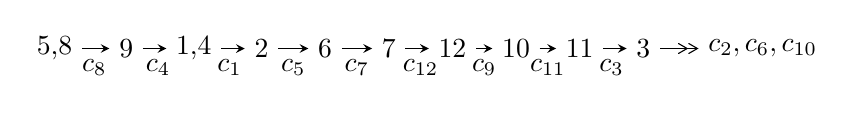
\begin{tikzpicture}[x=23pt, y=7pt]
	% node
	\node (A0) at (-1/8, 0) {5,8};
	\node (A1) at (1, 0) {9};
	\node (A2) at (33/16, 0) {1,4};
	\node (A3) at (25/8, 0) {2};
	\node (A4) at (33/8, 0) {6};
	\node (A5) at (41/8, 0) {7};
	\node (A6) at (49/8, 0) {12};
	\node (A7) at (57/8, 0) {10};
	\node (A8) at (65/8, 0) {11};
	\node (A9) at (73/8, 0) {3};
	\node (C1) at (1/2, -1) {$c_{8}$};
	\node (C2) at (3/2, -1) {$c_{4}$};
	\node (C3) at (21/8, -1) {$c_{1}$};
	\node (C4) at (29/8, -1) {$c_{5}$};
	\node (C5) at (37/8, -1) {$c_{7}$};
	\node (C6) at (45/8, -1) {$c_{12}$};
	\node (C7) at (53/8, -1) {$c_{9}$};
	\node (C8) at (61/8, -1) {$c_{11}$};
	\node (C9) at (69/8, -1) {$c_{3}$};
	\node (A10) at (11, 0) {$c_{2},c_{6},c_{10}$};

	% edge
	\draw[->,>=stealth]	
	(A0) edge (A1) (A1) edge (A2) (A2) edge (A3) (A3) edge (A4) (A4) edge (A5) (A5) edge (A6) (A6) edge (A7) (A7) edge (A8) (A8) edge (A9) ;
	\draw[->>,>={angle 60}]	
	(A9) edge (A10);
\end{tikzpicture} \\ 

\end{tabular} \\

\footnotetext{
The image of knot diagram is generated by the software ``\textbf{Draw programme}" developed by Andrew Bartholomew(\url{http://www.layer8.co.uk/maths/draw/index.htm\#Running-draw}), where we modified some parts for our purpose(\url{https://github.com/CATsTAILs/LinksPainter}).
}\phantom \\ \newline 
\centering \textbf{Ideals for irreducible components\footnotemark of $X_{\text{par}}$} 
 
\begin{align*}
I^u_{1}&=\langle 
1.43694\times10^{1247} u^{202}+6.99654\times10^{1246} u^{201}+\cdots+2.59373\times10^{1248} b-4.94103\times10^{1250},\\
\phantom{I^u_{1}}&\phantom{= \langle  }2.06789\times10^{1251} u^{202}+4.73176\times10^{1250} u^{201}+\cdots+1.89887\times10^{1252} a+5.27296\times10^{1254},\\
\phantom{I^u_{1}}&\phantom{= \langle  }u^{203}+2 u^{202}+\cdots-80511 u-7321\rangle \\
I^u_{2}&=\langle 
1.31314\times10^{60} u^{49}+1.32815\times10^{60} u^{48}+\cdots+7.86550\times10^{58} b+6.20943\times10^{59},\\
\phantom{I^u_{2}}&\phantom{= \langle  }-1.47583\times10^{60} u^{49}-1.56407\times10^{60} u^{48}+\cdots+7.86550\times10^{58} a-7.12810\times10^{59},\;u^{50}+u^{49}+\cdots- u+1\rangle \\
I^u_{3}&=\langle 
2 b-3,\;2 a+5,\;u-1\rangle \\
I^u_{4}&=\langle 
b,\;a+1,\;u-1\rangle \\
\\
\end{align*}
\raggedright * 4 irreducible components of $\dim_{\mathbb{C}}=0$, with total 255 representations.\\
\footnotetext{All coefficients of polynomials are rational numbers. But the coefficients are sometimes approximated in decimal forms when there is not enough margin.}
\newpage
\renewcommand{\arraystretch}{1}
\centering \section*{I. $I^u_{1}= \langle 1.44\times10^{1247} u^{202}+7.00\times10^{1246} u^{201}+\cdots+2.59\times10^{1248} b-4.94\times10^{1250},\;2.07\times10^{1251} u^{202}+4.73\times10^{1250} u^{201}+\cdots+1.90\times10^{1252} a+5.27\times10^{1254},\;u^{203}+2 u^{202}+\cdots-80511 u-7321 \rangle$}
\flushleft \textbf{(i) Arc colorings}\\
\begin{tabular}{m{7pt} m{180pt} m{7pt} m{180pt} }
\flushright $a_{5}=$&$\begin{pmatrix}0\\u\end{pmatrix}$ \\
\flushright $a_{8}=$&$\begin{pmatrix}1\\0\end{pmatrix}$ \\
\flushright $a_{9}=$&$\begin{pmatrix}1\\- u^2\end{pmatrix}$ \\
\flushright $a_{1}=$&$\begin{pmatrix}-0.108901 u^{202}-0.0249188 u^{201}+\cdots-1382.26 u-277.689\\-0.0554007 u^{202}-0.0269748 u^{201}+\cdots+2118.49 u+190.499\end{pmatrix}$ \\
\flushright $a_{4}=$&$\begin{pmatrix}- u\\u\end{pmatrix}$ \\
\flushright $a_{2}=$&$\begin{pmatrix}0.242892 u^{202}+0.297981 u^{201}+\cdots-22457.6 u-2303.48\\-0.407194 u^{202}-0.349875 u^{201}+\cdots+23193.8 u+2216.29\end{pmatrix}$ \\
\flushright $a_{6}=$&$\begin{pmatrix}0.205842 u^{202}+0.222492 u^{201}+\cdots-20845.4 u-2152.38\\-0.562734 u^{202}-0.554116 u^{201}+\cdots+41834.2 u+4150.50\end{pmatrix}$ \\
\flushright $a_{7}=$&$\begin{pmatrix}-0.408983 u^{202}-0.416467 u^{201}+\cdots+27287.1 u+2750.97\\0.227279 u^{202}+0.265027 u^{201}+\cdots-17597.8 u-1856.07\end{pmatrix}$ \\
\flushright $a_{12}=$&$\begin{pmatrix}0.200303 u^{202}+0.240294 u^{201}+\cdots-18232.7 u-1880.28\\-0.433780 u^{202}-0.408627 u^{201}+\cdots+28290.9 u+2776.24\end{pmatrix}$ \\
\flushright $a_{10}=$&$\begin{pmatrix}0.355570 u^{202}+0.433197 u^{201}+\cdots-31605.2 u-3205.28\\0.759767 u^{202}+0.907805 u^{201}+\cdots-65585.9 u-6627.87\end{pmatrix}$ \\
\flushright $a_{11}=$&$\begin{pmatrix}-1.63450 u^{202}-1.74050 u^{201}+\cdots+124864. u+12504.6\\1.60647 u^{202}+1.79540 u^{201}+\cdots-129709. u-13101.6\end{pmatrix}$ \\
\flushright $a_{3}=$&$\begin{pmatrix}0.321269 u^{202}+0.329106 u^{201}+\cdots-22483.3 u-2240.10\\0.389626 u^{202}+0.455494 u^{201}+\cdots-31040.9 u-3095.52\end{pmatrix}$\\&\end{tabular}
\flushleft \textbf{(ii) Obstruction class $= -1$}\\~\\
\flushleft \textbf{(iii) Cusp Shapes $= -12.4193 u^{202}-15.9063 u^{201}+\cdots+1.19388\times10^{6} u+123342.$}\\~\\
\newpage\renewcommand{\arraystretch}{1}
\flushleft \textbf{(iv) u-Polynomials at the component}\newline \\
\begin{tabular}{m{50pt}|m{274pt}}
Crossings & \hspace{64pt}u-Polynomials at each crossing \\
\hline $$\begin{aligned}c_{1}\end{aligned}$$&$\begin{aligned}
&u^{203}+10 u^{202}+\cdots-1413591 u+4819
\end{aligned}$\\
\hline $$\begin{aligned}c_{2}\end{aligned}$$&$\begin{aligned}
&u^{203}+3 u^{202}+\cdots+62 u+1
\end{aligned}$\\
\hline $$\begin{aligned}c_{3}\end{aligned}$$&$\begin{aligned}
&u^{203}+u^{202}+\cdots-274 u+16
\end{aligned}$\\
\hline $$\begin{aligned}c_{4},c_{8}\end{aligned}$$&$\begin{aligned}
&u^{203}-2 u^{202}+\cdots-80511 u+7321
\end{aligned}$\\
\hline $$\begin{aligned}c_{5}\end{aligned}$$&$\begin{aligned}
&2(2 u^{203}+u^{202}+\cdots-8.22687\times10^{10} u+4.61846\times10^{9})
\end{aligned}$\\
\hline $$\begin{aligned}c_{6}\end{aligned}$$&$\begin{aligned}
&2(2 u^{203}-7 u^{202}+\cdots+4 u+11)
\end{aligned}$\\
\hline $$\begin{aligned}c_{7}\end{aligned}$$&$\begin{aligned}
&2(2 u^{203}+5 u^{202}+\cdots+2459520 u+382966)
\end{aligned}$\\
\hline $$\begin{aligned}c_{9},c_{12}\end{aligned}$$&$\begin{aligned}
&u^{203}-8 u^{202}+\cdots-1110488 u+1091189
\end{aligned}$\\
\hline $$\begin{aligned}c_{10}\end{aligned}$$&$\begin{aligned}
&u^{203}-4 u^{201}+\cdots-1855 u+158
\end{aligned}$\\
\hline $$\begin{aligned}c_{11}\end{aligned}$$&$\begin{aligned}
&u^{203}+3 u^{202}+\cdots+6685893 u+3717382
\end{aligned}$\\
\hline
\end{tabular}\\~\\
\newpage\renewcommand{\arraystretch}{1}
\flushleft \textbf{(v) Riley Polynomials at the component}\newline \\
\begin{tabular}{m{50pt}|m{274pt}}
Crossings & \hspace{64pt}Riley Polynomials at each crossing \\
\hline $$\begin{aligned}c_{1}\end{aligned}$$&$\begin{aligned}
&y^{203}+42 y^{202}+\cdots+1989941534611 y-23222761
\end{aligned}$\\
\hline $$\begin{aligned}c_{2}\end{aligned}$$&$\begin{aligned}
&y^{203}+25 y^{202}+\cdots+194 y-1
\end{aligned}$\\
\hline $$\begin{aligned}c_{3}\end{aligned}$$&$\begin{aligned}
&y^{203}+9 y^{202}+\cdots+36740 y-256
\end{aligned}$\\
\hline $$\begin{aligned}c_{4},c_{8}\end{aligned}$$&$\begin{aligned}
&y^{203}-110 y^{202}+\cdots+5254435841 y-53597041
\end{aligned}$\\
\hline $$\begin{aligned}c_{5}\end{aligned}$$&$\begin{aligned}
&4(4 y^{203}-225 y^{202}+\cdots-1.19976\times10^{21} y-2.13302\times10^{19})
\end{aligned}$\\
\hline $$\begin{aligned}c_{6}\end{aligned}$$&$\begin{aligned}
&4(4 y^{203}-89 y^{202}+\cdots+3822 y-121)
\end{aligned}$\\
\hline $$\begin{aligned}c_{7}\end{aligned}$$&$\begin{aligned}
&4(4 y^{203}-49 y^{202}+\cdots+2.41353\times10^{12} y-1.46663\times10^{11})
\end{aligned}$\\
\hline $$\begin{aligned}c_{9},c_{12}\end{aligned}$$&$\begin{aligned}
&y^{203}+142 y^{202}+\cdots-192816319316354 y-1190693433721
\end{aligned}$\\
\hline $$\begin{aligned}c_{10}\end{aligned}$$&$\begin{aligned}
&y^{203}-8 y^{202}+\cdots+2071797 y-24964
\end{aligned}$\\
\hline $$\begin{aligned}c_{11}\end{aligned}$$&$\begin{aligned}
&y^{203}-19 y^{202}+\cdots+1958373122289601 y-13818928933924
\end{aligned}$\\
\hline
\end{tabular}\\~\\
\newpage\flushleft \textbf{(vi) Complex Volumes and Cusp Shapes}
$$\begin{array}{c|c|c}  
\text{Solutions to }I^u_{1}& \I (\text{vol} + \sqrt{-1}CS) & \text{Cusp shape}\\
 \hline 
\begin{aligned}
u &= -0.415362 + 0.899292 I \\
a &= -0.207812 + 0.662700 I \\
b &= -1.01362 - 1.05022 I\end{aligned}
 & -3.87742 + 6.13429 I & \phantom{-0.000000 } 0 \\ \hline\begin{aligned}
u &= -0.415362 - 0.899292 I \\
a &= -0.207812 - 0.662700 I \\
b &= -1.01362 + 1.05022 I\end{aligned}
 & -3.87742 - 6.13429 I & \phantom{-0.000000 } 0 \\ \hline\begin{aligned}
u &= -0.894875 + 0.420192 I \\
a &= \phantom{-}2.31810 - 0.46068 I \\
b &= -0.275272 + 0.760522 I\end{aligned}
 & -2.96780 - 12.19750 I & \phantom{-0.000000 } 0 \\ \hline\begin{aligned}
u &= -0.894875 - 0.420192 I \\
a &= \phantom{-}2.31810 + 0.46068 I \\
b &= -0.275272 - 0.760522 I\end{aligned}
 & -2.96780 + 12.19750 I & \phantom{-0.000000 } 0 \\ \hline\begin{aligned}
u &= \phantom{-}0.957452 + 0.245768 I \\
a &= -1.97389 - 1.04777 I \\
b &= \phantom{-}0.436871 + 0.247251 I\end{aligned}
 & \phantom{-}0.07450 + 5.23115 I & \phantom{-0.000000 } 0 \\ \hline\begin{aligned}
u &= \phantom{-}0.957452 - 0.245768 I \\
a &= -1.97389 + 1.04777 I \\
b &= \phantom{-}0.436871 - 0.247251 I\end{aligned}
 & \phantom{-}0.07450 - 5.23115 I & \phantom{-0.000000 } 0 \\ \hline\begin{aligned}
u &= -0.942656 + 0.291960 I \\
a &= \phantom{-}1.36836 + 1.40017 I \\
b &= -1.75070 - 1.53821 I\end{aligned}
 & -1.18988 - 1.42649 I & \phantom{-0.000000 } 0 \\ \hline\begin{aligned}
u &= -0.942656 - 0.291960 I \\
a &= \phantom{-}1.36836 - 1.40017 I \\
b &= -1.75070 + 1.53821 I\end{aligned}
 & -1.18988 + 1.42649 I & \phantom{-0.000000 } 0 \\ \hline\begin{aligned}
u &= -0.944282 + 0.280052 I \\
a &= -2.40162 + 0.54478 I \\
b &= \phantom{-}1.128980 - 0.281371 I\end{aligned}
 & -1.69095 - 4.88437 I & \phantom{-0.000000 } 0 \\ \hline\begin{aligned}
u &= -0.944282 - 0.280052 I \\
a &= -2.40162 - 0.54478 I \\
b &= \phantom{-}1.128980 + 0.281371 I\end{aligned}
 & -1.69095 + 4.88437 I & \phantom{-0.000000 } 0\\
 \hline 
 \end{array}$$\newpage$$\begin{array}{c|c|c}  
\text{Solutions to }I^u_{1}& \I (\text{vol} + \sqrt{-1}CS) & \text{Cusp shape}\\
 \hline 
\begin{aligned}
u &= -0.955121 + 0.229896 I \\
a &= -0.69761 + 1.69525 I \\
b &= \phantom{-}0.077342 + 0.607569 I\end{aligned}
 & -2.40362 - 6.14299 I & \phantom{-0.000000 } 0 \\ \hline\begin{aligned}
u &= -0.955121 - 0.229896 I \\
a &= -0.69761 - 1.69525 I \\
b &= \phantom{-}0.077342 - 0.607569 I\end{aligned}
 & -2.40362 + 6.14299 I & \phantom{-0.000000 } 0 \\ \hline\begin{aligned}
u &= \phantom{-}0.873412 + 0.437921 I \\
a &= -2.21088 + 0.44149 I \\
b &= \phantom{-}1.58276 + 0.07708 I\end{aligned}
 & -4.33235 + 7.06722 I & \phantom{-0.000000 } 0 \\ \hline\begin{aligned}
u &= \phantom{-}0.873412 - 0.437921 I \\
a &= -2.21088 - 0.44149 I \\
b &= \phantom{-}1.58276 - 0.07708 I\end{aligned}
 & -4.33235 - 7.06722 I & \phantom{-0.000000 } 0 \\ \hline\begin{aligned}
u &= -0.922495 + 0.317669 I \\
a &= \phantom{-}2.32477 - 0.59364 I \\
b &= -1.55662 + 0.79349 I\end{aligned}
 & -0.711081 + 0.821444 I & \phantom{-0.000000 } 0 \\ \hline\begin{aligned}
u &= -0.922495 - 0.317669 I \\
a &= \phantom{-}2.32477 + 0.59364 I \\
b &= -1.55662 - 0.79349 I\end{aligned}
 & -0.711081 - 0.821444 I & \phantom{-0.000000 } 0 \\ \hline\begin{aligned}
u &= -1.02967\phantom{ +0.000000I} \\
a &= -2.73050\phantom{ +0.000000I} \\
b &= \phantom{-}2.07191\phantom{ +0.000000I}\end{aligned}
 & \phantom{-}3.17175\phantom{ +0.000000I} & \phantom{-0.000000 } 0 \\ \hline\begin{aligned}
u &= \phantom{-}0.908540 + 0.485793 I \\
a &= \phantom{-}1.91311 + 0.40720 I \\
b &= -0.183286 - 0.925721 I\end{aligned}
 & -4.45106 + 3.58775 I & \phantom{-0.000000 } 0 \\ \hline\begin{aligned}
u &= \phantom{-}0.908540 - 0.485793 I \\
a &= \phantom{-}1.91311 - 0.40720 I \\
b &= -0.183286 + 0.925721 I\end{aligned}
 & -4.45106 - 3.58775 I & \phantom{-0.000000 } 0 \\ \hline\begin{aligned}
u &= \phantom{-}0.002924 + 0.969557 I \\
a &= \phantom{-}0.215865 - 0.353356 I \\
b &= -0.755237 - 0.103120 I\end{aligned}
 & \phantom{-}1.197420 + 0.343471 I & \phantom{-0.000000 } 0\\
 \hline 
 \end{array}$$\newpage$$\begin{array}{c|c|c}  
\text{Solutions to }I^u_{1}& \I (\text{vol} + \sqrt{-1}CS) & \text{Cusp shape}\\
 \hline 
\begin{aligned}
u &= \phantom{-}0.002924 - 0.969557 I \\
a &= \phantom{-}0.215865 + 0.353356 I \\
b &= -0.755237 + 0.103120 I\end{aligned}
 & \phantom{-}1.197420 - 0.343471 I & \phantom{-0.000000 } 0 \\ \hline\begin{aligned}
u &= \phantom{-}0.962951 + 0.368378 I \\
a &= \phantom{-}0.369831 - 0.789035 I \\
b &= -0.152701 - 0.978174 I\end{aligned}
 & -1.62798 + 3.27127 I & \phantom{-0.000000 } 0 \\ \hline\begin{aligned}
u &= \phantom{-}0.962951 - 0.368378 I \\
a &= \phantom{-}0.369831 + 0.789035 I \\
b &= -0.152701 + 0.978174 I\end{aligned}
 & -1.62798 - 3.27127 I & \phantom{-0.000000 } 0 \\ \hline\begin{aligned}
u &= -0.969947 + 0.369188 I \\
a &= \phantom{-}1.049870 + 0.082946 I \\
b &= -0.996577 + 0.501260 I\end{aligned}
 & \phantom{-}1.88034 - 0.84617 I & \phantom{-0.000000 } 0 \\ \hline\begin{aligned}
u &= -0.969947 - 0.369188 I \\
a &= \phantom{-}1.049870 - 0.082946 I \\
b &= -0.996577 - 0.501260 I\end{aligned}
 & \phantom{-}1.88034 + 0.84617 I & \phantom{-0.000000 } 0 \\ \hline\begin{aligned}
u &= \phantom{-}0.925121 + 0.470981 I \\
a &= -1.39409 - 0.32714 I \\
b &= \phantom{-}0.314429 - 0.093935 I\end{aligned}
 & -4.24178 + 5.99564 I & \phantom{-0.000000 } 0 \\ \hline\begin{aligned}
u &= \phantom{-}0.925121 - 0.470981 I \\
a &= -1.39409 + 0.32714 I \\
b &= \phantom{-}0.314429 + 0.093935 I\end{aligned}
 & -4.24178 - 5.99564 I & \phantom{-0.000000 } 0 \\ \hline\begin{aligned}
u &= -0.110478 + 0.947327 I \\
a &= -0.132327 - 0.741192 I \\
b &= -0.332324 + 0.434466 I\end{aligned}
 & -2.14005 - 2.25458 I & \phantom{-0.000000 } 0 \\ \hline\begin{aligned}
u &= -0.110478 - 0.947327 I \\
a &= -0.132327 + 0.741192 I \\
b &= -0.332324 - 0.434466 I\end{aligned}
 & -2.14005 + 2.25458 I & \phantom{-0.000000 } 0 \\ \hline\begin{aligned}
u &= \phantom{-}0.954179 + 0.433018 I \\
a &= \phantom{-}2.31534 + 0.68001 I \\
b &= -1.02239 - 1.44882 I\end{aligned}
 & -3.96433 + 2.21418 I & \phantom{-0.000000 } 0\\
 \hline 
 \end{array}$$\newpage$$\begin{array}{c|c|c}  
\text{Solutions to }I^u_{1}& \I (\text{vol} + \sqrt{-1}CS) & \text{Cusp shape}\\
 \hline 
\begin{aligned}
u &= \phantom{-}0.954179 - 0.433018 I \\
a &= \phantom{-}2.31534 - 0.68001 I \\
b &= -1.02239 + 1.44882 I\end{aligned}
 & -3.96433 - 2.21418 I & \phantom{-0.000000 } 0 \\ \hline\begin{aligned}
u &= -0.884096 + 0.332899 I \\
a &= -2.27083 + 1.15862 I \\
b &= \phantom{-}0.348050 - 1.059630 I\end{aligned}
 & -3.37792 - 2.31299 I & \phantom{-0.000000 } 0 \\ \hline\begin{aligned}
u &= -0.884096 - 0.332899 I \\
a &= -2.27083 - 1.15862 I \\
b &= \phantom{-}0.348050 + 1.059630 I\end{aligned}
 & -3.37792 + 2.31299 I & \phantom{-0.000000 } 0 \\ \hline\begin{aligned}
u &= \phantom{-}0.429512 + 0.967202 I \\
a &= \phantom{-}0.371661 + 0.539858 I \\
b &= \phantom{-}0.647467 - 0.921815 I\end{aligned}
 & -3.67535 - 0.55845 I & \phantom{-0.000000 } 0 \\ \hline\begin{aligned}
u &= \phantom{-}0.429512 - 0.967202 I \\
a &= \phantom{-}0.371661 - 0.539858 I \\
b &= \phantom{-}0.647467 + 0.921815 I\end{aligned}
 & -3.67535 + 0.55845 I & \phantom{-0.000000 } 0 \\ \hline\begin{aligned}
u &= \phantom{-}0.891779 + 0.268410 I \\
a &= \phantom{-}0.53167 - 1.78020 I \\
b &= -1.02805 + 2.30859 I\end{aligned}
 & -2.10369 + 11.24030 I & \phantom{-0.000000 } 0 \\ \hline\begin{aligned}
u &= \phantom{-}0.891779 - 0.268410 I \\
a &= \phantom{-}0.53167 + 1.78020 I \\
b &= -1.02805 - 2.30859 I\end{aligned}
 & -2.10369 - 11.24030 I & \phantom{-0.000000 } 0 \\ \hline\begin{aligned}
u &= -0.260923 + 1.047260 I \\
a &= \phantom{-}0.410929 + 0.209505 I \\
b &= \phantom{-}0.537624 - 0.746484 I\end{aligned}
 & -1.07835 - 6.96206 I & \phantom{-0.000000 } 0 \\ \hline\begin{aligned}
u &= -0.260923 - 1.047260 I \\
a &= \phantom{-}0.410929 - 0.209505 I \\
b &= \phantom{-}0.537624 + 0.746484 I\end{aligned}
 & -1.07835 + 6.96206 I & \phantom{-0.000000 } 0 \\ \hline\begin{aligned}
u &= -0.901398 + 0.148091 I \\
a &= -4.45131 + 0.77868 I \\
b &= \phantom{-}3.21285 - 0.84558 I\end{aligned}
 & -1.91204 - 0.43767 I & \phantom{-0.000000 } 0\\
 \hline 
 \end{array}$$\newpage$$\begin{array}{c|c|c}  
\text{Solutions to }I^u_{1}& \I (\text{vol} + \sqrt{-1}CS) & \text{Cusp shape}\\
 \hline 
\begin{aligned}
u &= -0.901398 - 0.148091 I \\
a &= -4.45131 - 0.77868 I \\
b &= \phantom{-}3.21285 + 0.84558 I\end{aligned}
 & -1.91204 + 0.43767 I & \phantom{-0.000000 } 0 \\ \hline\begin{aligned}
u &= \phantom{-}1.024860 + 0.385707 I \\
a &= \phantom{-}0.886805 - 0.318550 I \\
b &= -0.402786 - 0.843476 I\end{aligned}
 & -0.80214 + 3.54108 I & \phantom{-0.000000 } 0 \\ \hline\begin{aligned}
u &= \phantom{-}1.024860 - 0.385707 I \\
a &= \phantom{-}0.886805 + 0.318550 I \\
b &= -0.402786 + 0.843476 I\end{aligned}
 & -0.80214 - 3.54108 I & \phantom{-0.000000 } 0 \\ \hline\begin{aligned}
u &= -0.364898 + 0.817401 I \\
a &= -0.190010 - 0.027234 I \\
b &= -0.873020 - 0.277556 I\end{aligned}
 & \phantom{-}0.65598 + 1.89187 I & \phantom{-0.000000 } 0 \\ \hline\begin{aligned}
u &= -0.364898 - 0.817401 I \\
a &= -0.190010 + 0.027234 I \\
b &= -0.873020 + 0.277556 I\end{aligned}
 & \phantom{-}0.65598 - 1.89187 I & \phantom{-0.000000 } 0 \\ \hline\begin{aligned}
u &= \phantom{-}0.766108 + 0.454282 I \\
a &= \phantom{-}1.93240 + 0.48297 I \\
b &= -0.426037 - 0.609026 I\end{aligned}
 & -3.21700 - 1.11661 I & \phantom{-0.000000 } 0 \\ \hline\begin{aligned}
u &= \phantom{-}0.766108 - 0.454282 I \\
a &= \phantom{-}1.93240 - 0.48297 I \\
b &= -0.426037 + 0.609026 I\end{aligned}
 & -3.21700 + 1.11661 I & \phantom{-0.000000 } 0 \\ \hline\begin{aligned}
u &= \phantom{-}0.877362 + 0.121716 I \\
a &= \phantom{-}0.475549 + 0.912419 I \\
b &= -0.335112 + 1.041390 I\end{aligned}
 & -0.55840 - 3.52404 I & \phantom{-0.000000 } 0 \\ \hline\begin{aligned}
u &= \phantom{-}0.877362 - 0.121716 I \\
a &= \phantom{-}0.475549 - 0.912419 I \\
b &= -0.335112 - 1.041390 I\end{aligned}
 & -0.55840 + 3.52404 I & \phantom{-0.000000 } 0 \\ \hline\begin{aligned}
u &= \phantom{-}1.094060 + 0.220920 I \\
a &= -0.341521 + 1.071550 I \\
b &= \phantom{-}0.618269 - 0.016875 I\end{aligned}
 & \phantom{-}1.26413 - 3.68221 I & \phantom{-0.000000 } 0\\
 \hline 
 \end{array}$$\newpage$$\begin{array}{c|c|c}  
\text{Solutions to }I^u_{1}& \I (\text{vol} + \sqrt{-1}CS) & \text{Cusp shape}\\
 \hline 
\begin{aligned}
u &= \phantom{-}1.094060 - 0.220920 I \\
a &= -0.341521 - 1.071550 I \\
b &= \phantom{-}0.618269 + 0.016875 I\end{aligned}
 & \phantom{-}1.26413 + 3.68221 I & \phantom{-0.000000 } 0 \\ \hline\begin{aligned}
u &= \phantom{-}0.800482 + 0.361672 I \\
a &= -0.039714 + 0.229737 I \\
b &= \phantom{-}0.09793 - 1.43360 I\end{aligned}
 & -3.18474 + 4.65311 I & \phantom{-0.000000 } 0 \\ \hline\begin{aligned}
u &= \phantom{-}0.800482 - 0.361672 I \\
a &= -0.039714 - 0.229737 I \\
b &= \phantom{-}0.09793 + 1.43360 I\end{aligned}
 & -3.18474 - 4.65311 I & \phantom{-0.000000 } 0 \\ \hline\begin{aligned}
u &= \phantom{-}1.075270 + 0.330353 I \\
a &= -1.40397 + 0.83922 I \\
b &= \phantom{-}0.804313 + 0.822245 I\end{aligned}
 & \phantom{-}4.06060 + 2.22713 I & \phantom{-0.000000 } 0 \\ \hline\begin{aligned}
u &= \phantom{-}1.075270 - 0.330353 I \\
a &= -1.40397 - 0.83922 I \\
b &= \phantom{-}0.804313 - 0.822245 I\end{aligned}
 & \phantom{-}4.06060 - 2.22713 I & \phantom{-0.000000 } 0 \\ \hline\begin{aligned}
u &= \phantom{-}0.042996 + 0.873531 I \\
a &= -0.071817 + 0.645604 I \\
b &= \phantom{-}0.944670 + 0.424541 I\end{aligned}
 & \phantom{-}0.18540 + 10.12770 I & \phantom{-0.000000 } 0 \\ \hline\begin{aligned}
u &= \phantom{-}0.042996 - 0.873531 I \\
a &= -0.071817 - 0.645604 I \\
b &= \phantom{-}0.944670 - 0.424541 I\end{aligned}
 & \phantom{-}0.18540 - 10.12770 I & \phantom{-0.000000 } 0 \\ \hline\begin{aligned}
u &= -0.832254 + 0.246913 I \\
a &= -0.678227 + 0.454447 I \\
b &= -0.04173 - 1.90311 I\end{aligned}
 & -3.69799 - 0.33400 I & \phantom{-0.000000 } 0 \\ \hline\begin{aligned}
u &= -0.832254 - 0.246913 I \\
a &= -0.678227 - 0.454447 I \\
b &= -0.04173 + 1.90311 I\end{aligned}
 & -3.69799 + 0.33400 I & \phantom{-0.000000 } 0 \\ \hline\begin{aligned}
u &= \phantom{-}0.816391 + 0.287618 I \\
a &= -3.04409 - 0.84894 I \\
b &= \phantom{-}1.54769 + 0.98598 I\end{aligned}
 & -2.30645 - 8.68082 I & \phantom{-0.000000 } 0\\
 \hline 
 \end{array}$$\newpage$$\begin{array}{c|c|c}  
\text{Solutions to }I^u_{1}& \I (\text{vol} + \sqrt{-1}CS) & \text{Cusp shape}\\
 \hline 
\begin{aligned}
u &= \phantom{-}0.816391 - 0.287618 I \\
a &= -3.04409 + 0.84894 I \\
b &= \phantom{-}1.54769 - 0.98598 I\end{aligned}
 & -2.30645 + 8.68082 I & \phantom{-0.000000 } 0 \\ \hline\begin{aligned}
u &= -0.857881 + 0.074344 I \\
a &= -1.04252 - 3.43027 I \\
b &= \phantom{-}0.99926 + 3.69436 I\end{aligned}
 & -1.80683 - 2.95019 I & \phantom{-0.000000 } 0 \\ \hline\begin{aligned}
u &= -0.857881 - 0.074344 I \\
a &= -1.04252 + 3.43027 I \\
b &= \phantom{-}0.99926 - 3.69436 I\end{aligned}
 & -1.80683 + 2.95019 I & \phantom{-0.000000 } 0 \\ \hline\begin{aligned}
u &= -1.139700 + 0.067593 I \\
a &= -0.520122 - 1.027930 I \\
b &= \phantom{-}0.39701 + 1.50364 I\end{aligned}
 & \phantom{-}2.89468 - 0.55993 I & \phantom{-0.000000 } 0 \\ \hline\begin{aligned}
u &= -1.139700 - 0.067593 I \\
a &= -0.520122 + 1.027930 I \\
b &= \phantom{-}0.39701 - 1.50364 I\end{aligned}
 & \phantom{-}2.89468 + 0.55993 I & \phantom{-0.000000 } 0 \\ \hline\begin{aligned}
u &= \phantom{-}0.213387 + 1.122050 I \\
a &= -0.006654 - 0.400905 I \\
b &= -0.729469 + 0.863645 I\end{aligned}
 & -2.71993 - 6.98469 I & \phantom{-0.000000 } 0 \\ \hline\begin{aligned}
u &= \phantom{-}0.213387 - 1.122050 I \\
a &= -0.006654 + 0.400905 I \\
b &= -0.729469 - 0.863645 I\end{aligned}
 & -2.71993 + 6.98469 I & \phantom{-0.000000 } 0 \\ \hline\begin{aligned}
u &= \phantom{-}0.865936 + 0.759763 I \\
a &= -0.824712 + 1.043820 I \\
b &= \phantom{-}1.50845 + 0.02805 I\end{aligned}
 & \phantom{-}2.60381 - 2.66941 I & \phantom{-0.000000 } 0 \\ \hline\begin{aligned}
u &= \phantom{-}0.865936 - 0.759763 I \\
a &= -0.824712 - 1.043820 I \\
b &= \phantom{-}1.50845 - 0.02805 I\end{aligned}
 & \phantom{-}2.60381 + 2.66941 I & \phantom{-0.000000 } 0 \\ \hline\begin{aligned}
u &= -0.010172 + 0.845425 I \\
a &= -0.0798615 + 0.0371923 I \\
b &= -0.576223 + 0.925142 I\end{aligned}
 & -0.70649 - 4.59585 I & \phantom{-0.000000 } 0\\
 \hline 
 \end{array}$$\newpage$$\begin{array}{c|c|c}  
\text{Solutions to }I^u_{1}& \I (\text{vol} + \sqrt{-1}CS) & \text{Cusp shape}\\
 \hline 
\begin{aligned}
u &= -0.010172 - 0.845425 I \\
a &= -0.0798615 - 0.0371923 I \\
b &= -0.576223 - 0.925142 I\end{aligned}
 & -0.70649 + 4.59585 I & \phantom{-0.000000 } 0 \\ \hline\begin{aligned}
u &= \phantom{-}0.343191 + 1.103690 I \\
a &= -0.016323 + 0.159304 I \\
b &= \phantom{-}0.504999 - 0.890514 I\end{aligned}
 & -5.38825 - 3.22534 I & \phantom{-0.000000 } 0 \\ \hline\begin{aligned}
u &= \phantom{-}0.343191 - 1.103690 I \\
a &= -0.016323 - 0.159304 I \\
b &= \phantom{-}0.504999 + 0.890514 I\end{aligned}
 & -5.38825 + 3.22534 I & \phantom{-0.000000 } 0 \\ \hline\begin{aligned}
u &= -0.815581 + 0.185129 I \\
a &= \phantom{-}2.39613 - 1.59847 I \\
b &= -0.133508 - 0.163263 I\end{aligned}
 & -2.93557 + 4.13930 I & \phantom{-0.000000 } 0 \\ \hline\begin{aligned}
u &= -0.815581 - 0.185129 I \\
a &= \phantom{-}2.39613 + 1.59847 I \\
b &= -0.133508 + 0.163263 I\end{aligned}
 & -2.93557 - 4.13930 I & \phantom{-0.000000 } 0 \\ \hline\begin{aligned}
u &= \phantom{-}0.638771 + 0.534022 I \\
a &= \phantom{-}0.91341 - 1.16299 I \\
b &= -0.992251 + 0.995041 I\end{aligned}
 & -4.98129 - 3.10031 I & \phantom{-0.000000 } 0 \\ \hline\begin{aligned}
u &= \phantom{-}0.638771 - 0.534022 I \\
a &= \phantom{-}0.91341 + 1.16299 I \\
b &= -0.992251 - 0.995041 I\end{aligned}
 & -4.98129 + 3.10031 I & \phantom{-0.000000 } 0 \\ \hline\begin{aligned}
u &= -1.101910 + 0.395880 I \\
a &= \phantom{-}1.371280 + 0.233194 I \\
b &= -0.403056 + 0.715267 I\end{aligned}
 & \phantom{-}0.80956 + 1.89714 I & \phantom{-0.000000 } 0 \\ \hline\begin{aligned}
u &= -1.101910 - 0.395880 I \\
a &= \phantom{-}1.371280 - 0.233194 I \\
b &= -0.403056 - 0.715267 I\end{aligned}
 & \phantom{-}0.80956 - 1.89714 I & \phantom{-0.000000 } 0 \\ \hline\begin{aligned}
u &= -0.269452 + 0.780049 I \\
a &= \phantom{-}0.473111 + 0.407573 I \\
b &= -0.753563 + 0.404096 I\end{aligned}
 & \phantom{-}1.41980 - 1.71904 I & \phantom{-0.000000 } 0\\
 \hline 
 \end{array}$$\newpage$$\begin{array}{c|c|c}  
\text{Solutions to }I^u_{1}& \I (\text{vol} + \sqrt{-1}CS) & \text{Cusp shape}\\
 \hline 
\begin{aligned}
u &= -0.269452 - 0.780049 I \\
a &= \phantom{-}0.473111 - 0.407573 I \\
b &= -0.753563 - 0.404096 I\end{aligned}
 & \phantom{-}1.41980 + 1.71904 I & \phantom{-0.000000 } 0 \\ \hline\begin{aligned}
u &= -1.138150 + 0.299210 I \\
a &= \phantom{-}1.35093 + 0.62856 I \\
b &= -1.29931 + 0.77251 I\end{aligned}
 & \phantom{-}6.23829 + 1.55497 I & \phantom{-0.000000 } 0 \\ \hline\begin{aligned}
u &= -1.138150 - 0.299210 I \\
a &= \phantom{-}1.35093 - 0.62856 I \\
b &= -1.29931 - 0.77251 I\end{aligned}
 & \phantom{-}6.23829 - 1.55497 I & \phantom{-0.000000 } 0 \\ \hline\begin{aligned}
u &= \phantom{-}0.265605 + 1.147240 I \\
a &= \phantom{-}0.212614 + 0.344904 I \\
b &= \phantom{-}0.865737 - 0.876846 I\end{aligned}
 & -4.38293 - 6.78563 I & \phantom{-0.000000 } 0 \\ \hline\begin{aligned}
u &= \phantom{-}0.265605 - 1.147240 I \\
a &= \phantom{-}0.212614 - 0.344904 I \\
b &= \phantom{-}0.865737 + 0.876846 I\end{aligned}
 & -4.38293 + 6.78563 I & \phantom{-0.000000 } 0 \\ \hline\begin{aligned}
u &= -0.679012 + 0.462133 I \\
a &= \phantom{-}0.139102 + 0.479048 I \\
b &= \phantom{-}0.180311 + 1.399900 I\end{aligned}
 & -3.60861 + 8.48201 I & \phantom{-0.000000 } 0 \\ \hline\begin{aligned}
u &= -0.679012 - 0.462133 I \\
a &= \phantom{-}0.139102 - 0.479048 I \\
b &= \phantom{-}0.180311 - 1.399900 I\end{aligned}
 & -3.60861 - 8.48201 I & \phantom{-0.000000 } 0 \\ \hline\begin{aligned}
u &= -0.792909 + 0.204172 I \\
a &= \phantom{-}1.37194 + 0.46338 I \\
b &= -1.14683 - 1.24395 I\end{aligned}
 & -2.34259 + 2.56087 I & \phantom{-0.000000 } 0 \\ \hline\begin{aligned}
u &= -0.792909 - 0.204172 I \\
a &= \phantom{-}1.37194 - 0.46338 I \\
b &= -1.14683 + 1.24395 I\end{aligned}
 & -2.34259 - 2.56087 I & \phantom{-0.000000 } 0 \\ \hline\begin{aligned}
u &= -0.271401 + 1.154710 I \\
a &= \phantom{-}0.099871 - 0.368449 I \\
b &= \phantom{-}0.889741 + 0.903006 I\end{aligned}
 & -3.6186 + 15.5237 I & \phantom{-0.000000 } 0\\
 \hline 
 \end{array}$$\newpage$$\begin{array}{c|c|c}  
\text{Solutions to }I^u_{1}& \I (\text{vol} + \sqrt{-1}CS) & \text{Cusp shape}\\
 \hline 
\begin{aligned}
u &= -0.271401 - 1.154710 I \\
a &= \phantom{-}0.099871 + 0.368449 I \\
b &= \phantom{-}0.889741 - 0.903006 I\end{aligned}
 & -3.6186 - 15.5237 I & \phantom{-0.000000 } 0 \\ \hline\begin{aligned}
u &= -0.435292 + 1.111970 I \\
a &= \phantom{-}0.069919 + 0.485187 I \\
b &= -0.951304 - 0.672703 I\end{aligned}
 & -2.02991 + 5.84353 I & \phantom{-0.000000 } 0 \\ \hline\begin{aligned}
u &= -0.435292 - 1.111970 I \\
a &= \phantom{-}0.069919 - 0.485187 I \\
b &= -0.951304 + 0.672703 I\end{aligned}
 & -2.02991 - 5.84353 I & \phantom{-0.000000 } 0 \\ \hline\begin{aligned}
u &= \phantom{-}1.182400 + 0.190935 I \\
a &= -1.50368 + 0.33525 I \\
b &= \phantom{-}1.097070 + 0.323858 I\end{aligned}
 & \phantom{-}5.83772 + 0.71294 I & \phantom{-0.000000 } 0 \\ \hline\begin{aligned}
u &= \phantom{-}1.182400 - 0.190935 I \\
a &= -1.50368 - 0.33525 I \\
b &= \phantom{-}1.097070 - 0.323858 I\end{aligned}
 & \phantom{-}5.83772 - 0.71294 I & \phantom{-0.000000 } 0 \\ \hline\begin{aligned}
u &= -1.081480 + 0.537328 I \\
a &= -1.187790 - 0.745245 I \\
b &= \phantom{-}1.141800 - 0.682033 I\end{aligned}
 & \phantom{-}2.84415 - 6.88891 I & \phantom{-0.000000 } 0 \\ \hline\begin{aligned}
u &= -1.081480 - 0.537328 I \\
a &= -1.187790 + 0.745245 I \\
b &= \phantom{-}1.141800 + 0.682033 I\end{aligned}
 & \phantom{-}2.84415 + 6.88891 I & \phantom{-0.000000 } 0 \\ \hline\begin{aligned}
u &= \phantom{-}1.188680 + 0.256751 I \\
a &= \phantom{-}1.51320 - 0.22088 I \\
b &= -1.34257 - 0.86489 I\end{aligned}
 & \phantom{-}6.88601 + 7.01460 I & \phantom{-0.000000 } 0 \\ \hline\begin{aligned}
u &= \phantom{-}1.188680 - 0.256751 I \\
a &= \phantom{-}1.51320 + 0.22088 I \\
b &= -1.34257 + 0.86489 I\end{aligned}
 & \phantom{-}6.88601 - 7.01460 I & \phantom{-0.000000 } 0 \\ \hline\begin{aligned}
u &= -1.22377\phantom{ +0.000000I} \\
a &= \phantom{-}0.667574\phantom{ +0.000000I} \\
b &= -0.664785\phantom{ +0.000000I}\end{aligned}
 & \phantom{-}2.12975\phantom{ +0.000000I} & \phantom{-0.000000 } 0\\
 \hline 
 \end{array}$$\newpage$$\begin{array}{c|c|c}  
\text{Solutions to }I^u_{1}& \I (\text{vol} + \sqrt{-1}CS) & \text{Cusp shape}\\
 \hline 
\begin{aligned}
u &= \phantom{-}0.052728 + 0.773471 I \\
a &= \phantom{-}0.592347 - 0.222276 I \\
b &= \phantom{-}0.632140 + 0.717279 I\end{aligned}
 & \phantom{-}1.18303 - 1.12212 I & \phantom{-0.000000 } 0 \\ \hline\begin{aligned}
u &= \phantom{-}0.052728 - 0.773471 I \\
a &= \phantom{-}0.592347 + 0.222276 I \\
b &= \phantom{-}0.632140 - 0.717279 I\end{aligned}
 & \phantom{-}1.18303 + 1.12212 I & \phantom{-0.000000 } 0 \\ \hline\begin{aligned}
u &= \phantom{-}0.556308 + 0.530621 I \\
a &= \phantom{-}0.349625 - 0.423029 I \\
b &= \phantom{-}0.05029 - 1.42849 I\end{aligned}
 & -5.43601 + 0.55026 I & \phantom{-0.000000 } 0 \\ \hline\begin{aligned}
u &= \phantom{-}0.556308 - 0.530621 I \\
a &= \phantom{-}0.349625 + 0.423029 I \\
b &= \phantom{-}0.05029 + 1.42849 I\end{aligned}
 & -5.43601 - 0.55026 I & \phantom{-0.000000 } 0 \\ \hline\begin{aligned}
u &= \phantom{-}0.065083 + 0.765139 I \\
a &= \phantom{-}0.448016 - 0.636943 I \\
b &= \phantom{-}0.794968 - 0.365390 I\end{aligned}
 & -1.11795 - 3.00739 I & \phantom{-0.000000 } 0 \\ \hline\begin{aligned}
u &= \phantom{-}0.065083 - 0.765139 I \\
a &= \phantom{-}0.448016 + 0.636943 I \\
b &= \phantom{-}0.794968 + 0.365390 I\end{aligned}
 & -1.11795 + 3.00739 I & \phantom{-0.000000 } 0 \\ \hline\begin{aligned}
u &= \phantom{-}0.534570 + 0.538984 I \\
a &= \phantom{-}1.001020 + 0.057489 I \\
b &= -0.025673 + 0.876688 I\end{aligned}
 & -5.32769 - 1.89571 I & \phantom{-0.000000 } 0 \\ \hline\begin{aligned}
u &= \phantom{-}0.534570 - 0.538984 I \\
a &= \phantom{-}1.001020 - 0.057489 I \\
b &= -0.025673 - 0.876688 I\end{aligned}
 & -5.32769 + 1.89571 I & \phantom{-0.000000 } 0 \\ \hline\begin{aligned}
u &= \phantom{-}1.249960 + 0.086661 I \\
a &= -0.951881 + 0.548912 I \\
b &= \phantom{-}0.693915 + 0.234454 I\end{aligned}
 & \phantom{-}4.91107 - 2.60938 I & \phantom{-0.000000 } 0 \\ \hline\begin{aligned}
u &= \phantom{-}1.249960 - 0.086661 I \\
a &= -0.951881 - 0.548912 I \\
b &= \phantom{-}0.693915 - 0.234454 I\end{aligned}
 & \phantom{-}4.91107 + 2.60938 I & \phantom{-0.000000 } 0\\
 \hline 
 \end{array}$$\newpage$$\begin{array}{c|c|c}  
\text{Solutions to }I^u_{1}& \I (\text{vol} + \sqrt{-1}CS) & \text{Cusp shape}\\
 \hline 
\begin{aligned}
u &= -1.013070 + 0.753633 I \\
a &= -0.818664 - 0.742042 I \\
b &= \phantom{-}1.071270 + 0.063927 I\end{aligned}
 & \phantom{-}1.57323 - 4.08247 I & \phantom{-0.000000 } 0 \\ \hline\begin{aligned}
u &= -1.013070 - 0.753633 I \\
a &= -0.818664 + 0.742042 I \\
b &= \phantom{-}1.071270 - 0.063927 I\end{aligned}
 & \phantom{-}1.57323 + 4.08247 I & \phantom{-0.000000 } 0 \\ \hline\begin{aligned}
u &= \phantom{-}0.573407 + 0.450637 I \\
a &= \phantom{-}0.926937 + 0.857517 I \\
b &= \phantom{-}0.30459 - 1.77109 I\end{aligned}
 & -5.09680 + 1.51428 I & \phantom{-0.000000 } 0 \\ \hline\begin{aligned}
u &= \phantom{-}0.573407 - 0.450637 I \\
a &= \phantom{-}0.926937 - 0.857517 I \\
b &= \phantom{-}0.30459 + 1.77109 I\end{aligned}
 & -5.09680 - 1.51428 I & \phantom{-0.000000 } 0 \\ \hline\begin{aligned}
u &= -1.218510 + 0.433303 I \\
a &= \phantom{-}1.78226 - 0.25562 I \\
b &= -1.54961 + 1.20248 I\end{aligned}
 & \phantom{-}4.89627 - 3.18817 I & \phantom{-0.000000 } 0 \\ \hline\begin{aligned}
u &= -1.218510 - 0.433303 I \\
a &= \phantom{-}1.78226 + 0.25562 I \\
b &= -1.54961 - 1.20248 I\end{aligned}
 & \phantom{-}4.89627 + 3.18817 I & \phantom{-0.000000 } 0 \\ \hline\begin{aligned}
u &= \phantom{-}1.205960 + 0.471831 I \\
a &= \phantom{-}1.140010 - 0.464165 I \\
b &= -0.968014 - 0.917263 I\end{aligned}
 & \phantom{-}2.23510 + 7.55638 I & \phantom{-0.000000 } 0 \\ \hline\begin{aligned}
u &= \phantom{-}1.205960 - 0.471831 I \\
a &= \phantom{-}1.140010 + 0.464165 I \\
b &= -0.968014 + 0.917263 I\end{aligned}
 & \phantom{-}2.23510 - 7.55638 I & \phantom{-0.000000 } 0 \\ \hline\begin{aligned}
u &= \phantom{-}1.076910 + 0.731633 I \\
a &= \phantom{-}1.104930 - 0.772223 I \\
b &= -1.64432 - 0.24010 I\end{aligned}
 & \phantom{-}3.35185 + 8.56193 I & \phantom{-0.000000 } 0 \\ \hline\begin{aligned}
u &= \phantom{-}1.076910 - 0.731633 I \\
a &= \phantom{-}1.104930 + 0.772223 I \\
b &= -1.64432 + 0.24010 I\end{aligned}
 & \phantom{-}3.35185 - 8.56193 I & \phantom{-0.000000 } 0\\
 \hline 
 \end{array}$$\newpage$$\begin{array}{c|c|c}  
\text{Solutions to }I^u_{1}& \I (\text{vol} + \sqrt{-1}CS) & \text{Cusp shape}\\
 \hline 
\begin{aligned}
u &= \phantom{-}1.205910 + 0.499036 I \\
a &= \phantom{-}0.349419 - 0.637805 I \\
b &= -0.760091 - 0.280949 I\end{aligned}
 & \phantom{-}4.44591 + 5.77896 I & \phantom{-0.000000 } 0 \\ \hline\begin{aligned}
u &= \phantom{-}1.205910 - 0.499036 I \\
a &= \phantom{-}0.349419 + 0.637805 I \\
b &= -0.760091 + 0.280949 I\end{aligned}
 & \phantom{-}4.44591 - 5.77896 I & \phantom{-0.000000 } 0 \\ \hline\begin{aligned}
u &= -1.197130 + 0.521600 I \\
a &= \phantom{-}1.075450 + 0.236061 I \\
b &= -1.251450 + 0.306299 I\end{aligned}
 & \phantom{-}2.20417 - 1.19635 I & \phantom{-0.000000 } 0 \\ \hline\begin{aligned}
u &= -1.197130 - 0.521600 I \\
a &= \phantom{-}1.075450 - 0.236061 I \\
b &= -1.251450 - 0.306299 I\end{aligned}
 & \phantom{-}2.20417 + 1.19635 I & \phantom{-0.000000 } 0 \\ \hline\begin{aligned}
u &= \phantom{-}1.250610 + 0.403240 I \\
a &= -0.598433 - 0.572420 I \\
b &= \phantom{-}0.266291 + 1.274600 I\end{aligned}
 & \phantom{-}1.74199 + 9.64376 I & \phantom{-0.000000 } 0 \\ \hline\begin{aligned}
u &= \phantom{-}1.250610 - 0.403240 I \\
a &= -0.598433 + 0.572420 I \\
b &= \phantom{-}0.266291 - 1.274600 I\end{aligned}
 & \phantom{-}1.74199 - 9.64376 I & \phantom{-0.000000 } 0 \\ \hline\begin{aligned}
u &= \phantom{-}1.243750 + 0.426958 I \\
a &= -1.53999 - 0.22937 I \\
b &= \phantom{-}1.249270 + 0.627583 I\end{aligned}
 & \phantom{-}2.05540 + 6.79534 I & \phantom{-0.000000 } 0 \\ \hline\begin{aligned}
u &= \phantom{-}1.243750 - 0.426958 I \\
a &= -1.53999 + 0.22937 I \\
b &= \phantom{-}1.249270 - 0.627583 I\end{aligned}
 & \phantom{-}2.05540 - 6.79534 I & \phantom{-0.000000 } 0 \\ \hline\begin{aligned}
u &= -0.513289 + 1.211570 I \\
a &= -0.127132 - 0.366399 I \\
b &= \phantom{-}0.574258 + 0.642685 I\end{aligned}
 & -7.06711 - 3.23454 I & \phantom{-0.000000 } 0 \\ \hline\begin{aligned}
u &= -0.513289 - 1.211570 I \\
a &= -0.127132 + 0.366399 I \\
b &= \phantom{-}0.574258 - 0.642685 I\end{aligned}
 & -7.06711 + 3.23454 I & \phantom{-0.000000 } 0\\
 \hline 
 \end{array}$$\newpage$$\begin{array}{c|c|c}  
\text{Solutions to }I^u_{1}& \I (\text{vol} + \sqrt{-1}CS) & \text{Cusp shape}\\
 \hline 
\begin{aligned}
u &= \phantom{-}1.261240 + 0.393809 I \\
a &= -1.44998 + 0.40183 I \\
b &= \phantom{-}0.949217 + 0.670181 I\end{aligned}
 & \phantom{-}5.82658 + 5.77973 I & \phantom{-0.000000 } 0 \\ \hline\begin{aligned}
u &= \phantom{-}1.261240 - 0.393809 I \\
a &= -1.44998 - 0.40183 I \\
b &= \phantom{-}0.949217 - 0.670181 I\end{aligned}
 & \phantom{-}5.82658 - 5.77973 I & \phantom{-0.000000 } 0 \\ \hline\begin{aligned}
u &= -1.172960 + 0.613642 I \\
a &= -1.82281 - 0.14442 I \\
b &= \phantom{-}1.54599 - 1.12914 I\end{aligned}
 & -1.49415 - 11.74120 I & \phantom{-0.000000 } 0 \\ \hline\begin{aligned}
u &= -1.172960 - 0.613642 I \\
a &= -1.82281 + 0.14442 I \\
b &= \phantom{-}1.54599 + 1.12914 I\end{aligned}
 & -1.49415 + 11.74120 I & \phantom{-0.000000 } 0 \\ \hline\begin{aligned}
u &= \phantom{-}0.675643\phantom{ +0.000000I} \\
a &= -2.52107\phantom{ +0.000000I} \\
b &= -0.236846\phantom{ +0.000000I}\end{aligned}
 & \phantom{-}2.02655\phantom{ +0.000000I} & \phantom{-0.000000 } 0 \\ \hline\begin{aligned}
u &= \phantom{-}1.238130 + 0.473771 I \\
a &= -1.59437 - 0.18463 I \\
b &= \phantom{-}1.08643 + 1.18390 I\end{aligned}
 & \phantom{-}2.98501 + 9.30926 I & \phantom{-0.000000 } 0 \\ \hline\begin{aligned}
u &= \phantom{-}1.238130 - 0.473771 I \\
a &= -1.59437 + 0.18463 I \\
b &= \phantom{-}1.08643 - 1.18390 I\end{aligned}
 & \phantom{-}2.98501 - 9.30926 I & \phantom{-0.000000 } 0 \\ \hline\begin{aligned}
u &= -1.250080 + 0.465648 I \\
a &= \phantom{-}1.31986 + 0.54475 I \\
b &= -0.991665 + 0.829560 I\end{aligned}
 & \phantom{-}4.0376 - 14.8468 I & \phantom{-0.000000 } 0 \\ \hline\begin{aligned}
u &= -1.250080 - 0.465648 I \\
a &= \phantom{-}1.31986 - 0.54475 I \\
b &= -0.991665 - 0.829560 I\end{aligned}
 & \phantom{-}4.0376 + 14.8468 I & \phantom{-0.000000 } 0 \\ \hline\begin{aligned}
u &= -0.054257 + 0.661613 I \\
a &= -0.562765 + 0.865346 I \\
b &= \phantom{-}0.290493 + 0.871582 I\end{aligned}
 & -2.07189 - 5.72387 I & \phantom{-0.000000 } 0\\
 \hline 
 \end{array}$$\newpage$$\begin{array}{c|c|c}  
\text{Solutions to }I^u_{1}& \I (\text{vol} + \sqrt{-1}CS) & \text{Cusp shape}\\
 \hline 
\begin{aligned}
u &= -0.054257 - 0.661613 I \\
a &= -0.562765 - 0.865346 I \\
b &= \phantom{-}0.290493 - 0.871582 I\end{aligned}
 & -2.07189 + 5.72387 I & \phantom{-0.000000 } 0 \\ \hline\begin{aligned}
u &= \phantom{-}1.179620 + 0.636565 I \\
a &= \phantom{-}1.393230 - 0.006450 I \\
b &= -1.22409 - 1.11680 I\end{aligned}
 & -1.29940 + 6.41396 I & \phantom{-0.000000 } 0 \\ \hline\begin{aligned}
u &= \phantom{-}1.179620 - 0.636565 I \\
a &= \phantom{-}1.393230 + 0.006450 I \\
b &= -1.22409 + 1.11680 I\end{aligned}
 & -1.29940 - 6.41396 I & \phantom{-0.000000 } 0 \\ \hline\begin{aligned}
u &= -1.274130 + 0.427777 I \\
a &= -0.390987 - 0.214331 I \\
b &= \phantom{-}0.223897 - 0.703435 I\end{aligned}
 & \phantom{-}1.83991 - 2.95394 I & \phantom{-0.000000 } 0 \\ \hline\begin{aligned}
u &= -1.274130 - 0.427777 I \\
a &= -0.390987 + 0.214331 I \\
b &= \phantom{-}0.223897 + 0.703435 I\end{aligned}
 & \phantom{-}1.83991 + 2.95394 I & \phantom{-0.000000 } 0 \\ \hline\begin{aligned}
u &= -0.607400 + 0.219072 I \\
a &= -2.91038 - 1.07849 I \\
b &= \phantom{-}1.023400 + 0.374254 I\end{aligned}
 & -2.50491 - 0.93914 I & \phantom{-0.000000 } 0 \\ \hline\begin{aligned}
u &= -0.607400 - 0.219072 I \\
a &= -2.91038 + 1.07849 I \\
b &= \phantom{-}1.023400 - 0.374254 I\end{aligned}
 & -2.50491 + 0.93914 I & \phantom{-0.000000 } 0 \\ \hline\begin{aligned}
u &= \phantom{-}1.282490 + 0.448602 I \\
a &= -1.327440 + 0.245431 I \\
b &= \phantom{-}1.055040 + 0.280830 I\end{aligned}
 & \phantom{-}5.31228 + 4.65426 I & \phantom{-0.000000 } 0 \\ \hline\begin{aligned}
u &= \phantom{-}1.282490 - 0.448602 I \\
a &= -1.327440 - 0.245431 I \\
b &= \phantom{-}1.055040 - 0.280830 I\end{aligned}
 & \phantom{-}5.31228 - 4.65426 I & \phantom{-0.000000 } 0 \\ \hline\begin{aligned}
u &= -1.281500 + 0.461344 I \\
a &= -1.164950 - 0.538206 I \\
b &= \phantom{-}0.874887 - 0.510887 I\end{aligned}
 & \phantom{-}5.24555 - 5.35358 I & \phantom{-0.000000 } 0\\
 \hline 
 \end{array}$$\newpage$$\begin{array}{c|c|c}  
\text{Solutions to }I^u_{1}& \I (\text{vol} + \sqrt{-1}CS) & \text{Cusp shape}\\
 \hline 
\begin{aligned}
u &= -1.281500 - 0.461344 I \\
a &= -1.164950 + 0.538206 I \\
b &= \phantom{-}0.874887 + 0.510887 I\end{aligned}
 & \phantom{-}5.24555 + 5.35358 I & \phantom{-0.000000 } 0 \\ \hline\begin{aligned}
u &= \phantom{-}1.303080 + 0.416173 I \\
a &= \phantom{-}1.62422 + 0.48159 I \\
b &= -1.50793 - 1.26810 I\end{aligned}
 & \phantom{-}3.73766 + 11.68480 I & \phantom{-0.000000 } 0 \\ \hline\begin{aligned}
u &= \phantom{-}1.303080 - 0.416173 I \\
a &= \phantom{-}1.62422 - 0.48159 I \\
b &= -1.50793 + 1.26810 I\end{aligned}
 & \phantom{-}3.73766 - 11.68480 I & \phantom{-0.000000 } 0 \\ \hline\begin{aligned}
u &= -1.304420 + 0.454028 I \\
a &= -0.141883 - 0.461984 I \\
b &= \phantom{-}0.318072 + 0.042269 I\end{aligned}
 & \phantom{-}3.07900 - 0.31827 I & \phantom{-0.000000 } 0 \\ \hline\begin{aligned}
u &= -1.304420 - 0.454028 I \\
a &= -0.141883 + 0.461984 I \\
b &= \phantom{-}0.318072 - 0.042269 I\end{aligned}
 & \phantom{-}3.07900 + 0.31827 I & \phantom{-0.000000 } 0 \\ \hline\begin{aligned}
u &= \phantom{-}1.230340 + 0.637651 I \\
a &= \phantom{-}1.41504 - 0.03909 I \\
b &= -0.926259 - 0.968381 I\end{aligned}
 & -2.54772 + 9.37229 I & \phantom{-0.000000 } 0 \\ \hline\begin{aligned}
u &= \phantom{-}1.230340 - 0.637651 I \\
a &= \phantom{-}1.41504 + 0.03909 I \\
b &= -0.926259 + 0.968381 I\end{aligned}
 & -2.54772 - 9.37229 I & \phantom{-0.000000 } 0 \\ \hline\begin{aligned}
u &= \phantom{-}1.307890 + 0.491037 I \\
a &= \phantom{-}0.976124 - 0.441253 I \\
b &= -1.132070 + 0.084049 I\end{aligned}
 & \phantom{-}3.92694 - 5.04300 I & \phantom{-0.000000 } 0 \\ \hline\begin{aligned}
u &= \phantom{-}1.307890 - 0.491037 I \\
a &= \phantom{-}0.976124 + 0.441253 I \\
b &= -1.132070 - 0.084049 I\end{aligned}
 & \phantom{-}3.92694 + 5.04300 I & \phantom{-0.000000 } 0 \\ \hline\begin{aligned}
u &= -1.223770 + 0.679062 I \\
a &= \phantom{-}1.347210 + 0.039797 I \\
b &= -1.051200 + 0.826646 I\end{aligned}
 & -4.54322 - 3.37296 I & \phantom{-0.000000 } 0\\
 \hline 
 \end{array}$$\newpage$$\begin{array}{c|c|c}  
\text{Solutions to }I^u_{1}& \I (\text{vol} + \sqrt{-1}CS) & \text{Cusp shape}\\
 \hline 
\begin{aligned}
u &= -1.223770 - 0.679062 I \\
a &= \phantom{-}1.347210 - 0.039797 I \\
b &= -1.051200 - 0.826646 I\end{aligned}
 & -4.54322 + 3.37296 I & \phantom{-0.000000 } 0 \\ \hline\begin{aligned}
u &= -1.406340 + 0.080162 I \\
a &= \phantom{-}0.594314 + 0.235923 I \\
b &= -0.839831 + 0.337638 I\end{aligned}
 & \phantom{-}2.38224 + 2.06034 I & \phantom{-0.000000 } 0 \\ \hline\begin{aligned}
u &= -1.406340 - 0.080162 I \\
a &= \phantom{-}0.594314 - 0.235923 I \\
b &= -0.839831 - 0.337638 I\end{aligned}
 & \phantom{-}2.38224 - 2.06034 I & \phantom{-0.000000 } 0 \\ \hline\begin{aligned}
u &= -1.40691 + 0.15993 I \\
a &= -0.372017 - 0.543088 I \\
b &= \phantom{-}0.308061 - 0.099331 I\end{aligned}
 & \phantom{-}3.53879 + 2.13558 I & \phantom{-0.000000 } 0 \\ \hline\begin{aligned}
u &= -1.40691 - 0.15993 I \\
a &= -0.372017 + 0.543088 I \\
b &= \phantom{-}0.308061 + 0.099331 I\end{aligned}
 & \phantom{-}3.53879 - 2.13558 I & \phantom{-0.000000 } 0 \\ \hline\begin{aligned}
u &= -1.24401 + 0.68372 I \\
a &= -1.48786 - 0.24785 I \\
b &= \phantom{-}1.39493 - 0.83989 I\end{aligned}
 & \phantom{-}0.61012 - 12.28850 I & \phantom{-0.000000 } 0 \\ \hline\begin{aligned}
u &= -1.24401 - 0.68372 I \\
a &= -1.48786 + 0.24785 I \\
b &= \phantom{-}1.39493 + 0.83989 I\end{aligned}
 & \phantom{-}0.61012 + 12.28850 I & \phantom{-0.000000 } 0 \\ \hline\begin{aligned}
u &= \phantom{-}1.28716 + 0.61038 I \\
a &= -1.57905 - 0.04886 I \\
b &= \phantom{-}1.30729 + 1.04740 I\end{aligned}
 & \phantom{-}0.67097 + 13.08400 I & \phantom{-0.000000 } 0 \\ \hline\begin{aligned}
u &= \phantom{-}1.28716 - 0.61038 I \\
a &= -1.57905 + 0.04886 I \\
b &= \phantom{-}1.30729 - 1.04740 I\end{aligned}
 & \phantom{-}0.67097 - 13.08400 I & \phantom{-0.000000 } 0 \\ \hline\begin{aligned}
u &= \phantom{-}0.513258 + 0.251212 I \\
a &= \phantom{-}2.83960 - 0.23058 I \\
b &= \phantom{-}0.073077 - 0.169275 I\end{aligned}
 & -2.97053 - 0.15806 I & \phantom{-0.000000 } 0\\
 \hline 
 \end{array}$$\newpage$$\begin{array}{c|c|c}  
\text{Solutions to }I^u_{1}& \I (\text{vol} + \sqrt{-1}CS) & \text{Cusp shape}\\
 \hline 
\begin{aligned}
u &= \phantom{-}0.513258 - 0.251212 I \\
a &= \phantom{-}2.83960 + 0.23058 I \\
b &= \phantom{-}0.073077 + 0.169275 I\end{aligned}
 & -2.97053 + 0.15806 I & \phantom{-0.000000 } 0 \\ \hline\begin{aligned}
u &= \phantom{-}1.28306 + 0.63744 I \\
a &= \phantom{-}1.53530 - 0.00970 I \\
b &= -1.36477 - 1.22866 I\end{aligned}
 & -1.14839 + 13.07000 I & \phantom{-0.000000 } 0 \\ \hline\begin{aligned}
u &= \phantom{-}1.28306 - 0.63744 I \\
a &= \phantom{-}1.53530 + 0.00970 I \\
b &= -1.36477 + 1.22866 I\end{aligned}
 & -1.14839 - 13.07000 I & \phantom{-0.000000 } 0 \\ \hline\begin{aligned}
u &= -1.40372 + 0.31591 I \\
a &= -0.792881 + 0.800536 I \\
b &= \phantom{-}0.577716 - 1.230100 I\end{aligned}
 & \phantom{-}1.38175 - 1.95752 I & \phantom{-0.000000 } 0 \\ \hline\begin{aligned}
u &= -1.40372 - 0.31591 I \\
a &= -0.792881 - 0.800536 I \\
b &= \phantom{-}0.577716 + 1.230100 I\end{aligned}
 & \phantom{-}1.38175 + 1.95752 I & \phantom{-0.000000 } 0 \\ \hline\begin{aligned}
u &= -1.28698 + 0.64633 I \\
a &= \phantom{-}1.58437 + 0.03359 I \\
b &= -1.37421 + 1.16127 I\end{aligned}
 & -0.3936 - 21.8727 I & \phantom{-0.000000 } 0 \\ \hline\begin{aligned}
u &= -1.28698 - 0.64633 I \\
a &= \phantom{-}1.58437 - 0.03359 I \\
b &= -1.37421 - 1.16127 I\end{aligned}
 & -0.3936 + 21.8727 I & \phantom{-0.000000 } 0 \\ \hline\begin{aligned}
u &= \phantom{-}0.35989 + 1.41070 I \\
a &= -0.007257 - 0.355529 I \\
b &= -0.529463 + 0.529576 I\end{aligned}
 & -6.59977 - 4.77761 I & \phantom{-0.000000 } 0 \\ \hline\begin{aligned}
u &= \phantom{-}0.35989 - 1.41070 I \\
a &= -0.007257 + 0.355529 I \\
b &= -0.529463 - 0.529576 I\end{aligned}
 & -6.59977 + 4.77761 I & \phantom{-0.000000 } 0 \\ \hline\begin{aligned}
u &= -1.11486 + 0.95215 I \\
a &= -0.668965 - 0.460897 I \\
b &= \phantom{-}1.003180 - 0.449210 I\end{aligned}
 & \phantom{-}1.88854 - 6.49373 I & \phantom{-0.000000 } 0\\
 \hline 
 \end{array}$$\newpage$$\begin{array}{c|c|c}  
\text{Solutions to }I^u_{1}& \I (\text{vol} + \sqrt{-1}CS) & \text{Cusp shape}\\
 \hline 
\begin{aligned}
u &= -1.11486 - 0.95215 I \\
a &= -0.668965 + 0.460897 I \\
b &= \phantom{-}1.003180 + 0.449210 I\end{aligned}
 & \phantom{-}1.88854 + 6.49373 I & \phantom{-0.000000 } 0 \\ \hline\begin{aligned}
u &= \phantom{-}0.303556 + 0.437243 I \\
a &= \phantom{-}1.19782 - 1.34934 I \\
b &= \phantom{-}0.167026 - 0.477971 I\end{aligned}
 & -2.66082 + 0.01005 I & \phantom{-0.000000 } 0 \\ \hline\begin{aligned}
u &= \phantom{-}0.303556 - 0.437243 I \\
a &= \phantom{-}1.19782 + 1.34934 I \\
b &= \phantom{-}0.167026 + 0.477971 I\end{aligned}
 & -2.66082 - 0.01005 I & \phantom{-0.000000 } 0 \\ \hline\begin{aligned}
u &= \phantom{-}1.33693 + 0.69360 I \\
a &= -1.179050 - 0.079614 I \\
b &= \phantom{-}1.07542 + 0.94938 I\end{aligned}
 & -3.23328 + 11.93110 I & \phantom{-0.000000 } 0 \\ \hline\begin{aligned}
u &= \phantom{-}1.33693 - 0.69360 I \\
a &= -1.179050 + 0.079614 I \\
b &= \phantom{-}1.07542 - 0.94938 I\end{aligned}
 & -3.23328 - 11.93110 I & \phantom{-0.000000 } 0 \\ \hline\begin{aligned}
u &= -1.39782 + 0.58166 I \\
a &= -0.903378 - 0.227842 I \\
b &= \phantom{-}0.782382 - 0.184890 I\end{aligned}
 & \phantom{-}4.32382 - 4.36197 I & \phantom{-0.000000 } 0 \\ \hline\begin{aligned}
u &= -1.39782 - 0.58166 I \\
a &= -0.903378 + 0.227842 I \\
b &= \phantom{-}0.782382 + 0.184890 I\end{aligned}
 & \phantom{-}4.32382 + 4.36197 I & \phantom{-0.000000 } 0 \\ \hline\begin{aligned}
u &= -1.29354 + 0.80196 I \\
a &= \phantom{-}0.740786 + 0.262010 I \\
b &= -1.127660 + 0.333991 I\end{aligned}
 & \phantom{-}2.74824 - 1.18727 I & \phantom{-0.000000 } 0 \\ \hline\begin{aligned}
u &= -1.29354 - 0.80196 I \\
a &= \phantom{-}0.740786 - 0.262010 I \\
b &= -1.127660 - 0.333991 I\end{aligned}
 & \phantom{-}2.74824 + 1.18727 I & \phantom{-0.000000 } 0 \\ \hline\begin{aligned}
u &= \phantom{-}1.52314 + 0.09990 I \\
a &= \phantom{-}0.472288 - 0.431171 I \\
b &= -0.627983 - 0.061840 I\end{aligned}
 & \phantom{-}3.13305 - 10.50110 I & \phantom{-0.000000 } 0\\
 \hline 
 \end{array}$$\newpage$$\begin{array}{c|c|c}  
\text{Solutions to }I^u_{1}& \I (\text{vol} + \sqrt{-1}CS) & \text{Cusp shape}\\
 \hline 
\begin{aligned}
u &= \phantom{-}1.52314 - 0.09990 I \\
a &= \phantom{-}0.472288 + 0.431171 I \\
b &= -0.627983 + 0.061840 I\end{aligned}
 & \phantom{-}3.13305 + 10.50110 I & \phantom{-0.000000 } 0 \\ \hline\begin{aligned}
u &= -0.070900 + 0.462386 I \\
a &= \phantom{-}1.66475 - 0.10332 I \\
b &= \phantom{-}0.952118 - 0.119605 I\end{aligned}
 & \phantom{-}3.12794 - 4.43449 I & \phantom{-}8.44885 + 7.26104 I \\ \hline\begin{aligned}
u &= -0.070900 - 0.462386 I \\
a &= \phantom{-}1.66475 + 0.10332 I \\
b &= \phantom{-}0.952118 + 0.119605 I\end{aligned}
 & \phantom{-}3.12794 + 4.43449 I & \phantom{-}8.44885 - 7.26104 I \\ \hline\begin{aligned}
u &= -1.53994 + 0.42816 I \\
a &= \phantom{-}0.020260 + 0.262022 I \\
b &= -0.278160 + 0.314783 I\end{aligned}
 & \phantom{-}3.08513 + 0.35535 I & \phantom{-0.000000 } 0 \\ \hline\begin{aligned}
u &= -1.53994 - 0.42816 I \\
a &= \phantom{-}0.020260 - 0.262022 I \\
b &= -0.278160 - 0.314783 I\end{aligned}
 & \phantom{-}3.08513 - 0.35535 I & \phantom{-0.000000 } 0 \\ \hline\begin{aligned}
u &= -0.103713 + 0.387544 I \\
a &= \phantom{-}1.199040 - 0.357427 I \\
b &= -0.117582 + 0.482643 I\end{aligned}
 & \phantom{-}0.444059 - 1.261860 I & \phantom{-}4.91286 + 4.63218 I \\ \hline\begin{aligned}
u &= -0.103713 - 0.387544 I \\
a &= \phantom{-}1.199040 + 0.357427 I \\
b &= -0.117582 - 0.482643 I\end{aligned}
 & \phantom{-}0.444059 + 1.261860 I & \phantom{-}4.91286 - 4.63218 I \\ \hline\begin{aligned}
u &= -0.07668 + 1.64017 I \\
a &= -0.065784 + 0.228145 I \\
b &= -0.152486 - 0.228209 I\end{aligned}
 & -4.67638 - 4.52811 I & \phantom{-0.000000 } 0 \\ \hline\begin{aligned}
u &= -0.07668 - 1.64017 I \\
a &= -0.065784 - 0.228145 I \\
b &= -0.152486 + 0.228209 I\end{aligned}
 & -4.67638 + 4.52811 I & \phantom{-0.000000 } 0 \\ \hline\begin{aligned}
u &= -0.110178 + 0.330566 I \\
a &= \phantom{-}1.16392 - 0.98764 I \\
b &= -0.109711 + 1.282780 I\end{aligned}
 & -2.39619 - 3.50536 I & -2.32903 + 1.77977 I\\
 \hline 
 \end{array}$$\newpage$$\begin{array}{c|c|c}  
\text{Solutions to }I^u_{1}& \I (\text{vol} + \sqrt{-1}CS) & \text{Cusp shape}\\
 \hline 
\begin{aligned}
u &= -0.110178 - 0.330566 I \\
a &= \phantom{-}1.16392 + 0.98764 I \\
b &= -0.109711 - 1.282780 I\end{aligned}
 & -2.39619 + 3.50536 I & -2.32903 - 1.77977 I \\ \hline\begin{aligned}
u &= -0.229828\phantom{ +0.000000I} \\
a &= \phantom{-}1.78238\phantom{ +0.000000I} \\
b &= -0.776172\phantom{ +0.000000I}\end{aligned}
 & \phantom{-}1.64369\phantom{ +0.000000I} & \phantom{-}8.11750\phantom{ +0.000000I} \\ \hline\begin{aligned}
u &= -0.129423\phantom{ +0.000000I} \\
a &= \phantom{-}5.65008\phantom{ +0.000000I} \\
b &= -0.896993\phantom{ +0.000000I}\end{aligned}
 & \phantom{-}1.59226\phantom{ +0.000000I} & \phantom{-}11.9420\phantom{ +0.000000I}\\
 \hline 
 \end{array}$$\newpage\newpage\renewcommand{\arraystretch}{1}
\centering \section*{II. $I^u_{2}= \langle 1.31\times10^{60} u^{49}+1.33\times10^{60} u^{48}+\cdots+7.87\times10^{58} b+6.21\times10^{59},\;-1.48\times10^{60} u^{49}-1.56\times10^{60} u^{48}+\cdots+7.87\times10^{58} a-7.13\times10^{59},\;u^{50}+u^{49}+\cdots- u+1 \rangle$}
\flushleft \textbf{(i) Arc colorings}\\
\begin{tabular}{m{7pt} m{180pt} m{7pt} m{180pt} }
\flushright $a_{5}=$&$\begin{pmatrix}0\\u\end{pmatrix}$ \\
\flushright $a_{8}=$&$\begin{pmatrix}1\\0\end{pmatrix}$ \\
\flushright $a_{9}=$&$\begin{pmatrix}1\\- u^2\end{pmatrix}$ \\
\flushright $a_{1}=$&$\begin{pmatrix}18.7634 u^{49}+19.8851 u^{48}+\cdots-48.5576 u+9.06249\\-16.6950 u^{49}-16.8858 u^{48}+\cdots+41.3570 u-7.89452\end{pmatrix}$ \\
\flushright $a_{4}=$&$\begin{pmatrix}- u\\u\end{pmatrix}$ \\
\flushright $a_{2}=$&$\begin{pmatrix}17.6370 u^{49}+18.2744 u^{48}+\cdots-47.4202 u+9.99346\\-15.5686 u^{49}-15.2750 u^{48}+\cdots+40.2196 u-8.82549\end{pmatrix}$ \\
\flushright $a_{6}=$&$\begin{pmatrix}21.0483 u^{49}-10.5923 u^{48}+\cdots-127.437 u+67.3379\\-12.4036 u^{49}+10.1549 u^{48}+\cdots+73.6768 u-43.7186\end{pmatrix}$ \\
\flushright $a_{7}=$&$\begin{pmatrix}-60.9798 u^{49}-45.6514 u^{48}+\cdots+182.212 u-46.5606\\39.1711 u^{49}+33.8004 u^{48}+\cdots-95.6716 u+16.8798\end{pmatrix}$ \\
\flushright $a_{12}=$&$\begin{pmatrix}24.9094 u^{49}+23.6681 u^{48}+\cdots-72.2730 u+18.0788\\-19.9736 u^{49}-19.6660 u^{48}+\cdots+49.8661 u-10.2575\end{pmatrix}$ \\
\flushright $a_{10}=$&$\begin{pmatrix}22.7887 u^{49}+14.0600 u^{48}+\cdots-58.8778 u+17.1876\\-4.76674 u^{49}-11.2406 u^{48}+\cdots-1.30878 u+9.26784\end{pmatrix}$ \\
\flushright $a_{11}=$&$\begin{pmatrix}-41.0336 u^{49}-47.5575 u^{48}+\cdots+99.1207 u-20.2116\\39.3074 u^{49}+44.7248 u^{48}+\cdots-77.7751 u+14.1418\end{pmatrix}$ \\
\flushright $a_{3}=$&$\begin{pmatrix}-49.3553 u^{49}-5.70787 u^{48}+\cdots+169.775 u-83.7004\\21.4885 u^{49}-4.89438 u^{48}+\cdots-64.3359 u+39.9719\end{pmatrix}$\\&\end{tabular}
\flushleft \textbf{(ii) Obstruction class $= 1$}\\~\\
\flushleft \textbf{(iii) Cusp Shapes $= 300.545 u^{49}+408.122 u^{48}+\cdots-390.330 u-108.565$}\\~\\
\newpage\renewcommand{\arraystretch}{1}
\flushleft \textbf{(iv) u-Polynomials at the component}\newline \\
\begin{tabular}{m{50pt}|m{274pt}}
Crossings & \hspace{64pt}u-Polynomials at each crossing \\
\hline $$\begin{aligned}c_{1}\end{aligned}$$&$\begin{aligned}
&u^{50}-15 u^{49}+\cdots-5 u+1
\end{aligned}$\\
\hline $$\begin{aligned}c_{2}\end{aligned}$$&$\begin{aligned}
&u^{50}+2 u^{49}+\cdots+8 u+1
\end{aligned}$\\
\hline $$\begin{aligned}c_{3}\end{aligned}$$&$\begin{aligned}
&u^{50}+2 u^{49}+\cdots+152 u+9
\end{aligned}$\\
\hline $$\begin{aligned}c_{4}\end{aligned}$$&$\begin{aligned}
&u^{50}- u^{49}+\cdots+u+1
\end{aligned}$\\
\hline $$\begin{aligned}c_{5}\end{aligned}$$&$\begin{aligned}
&u^{50}+3 u^{49}+\cdots+62 u+3
\end{aligned}$\\
\hline $$\begin{aligned}c_{6}\end{aligned}$$&$\begin{aligned}
&u^{50}+4 u^{49}+\cdots-7 u+1
\end{aligned}$\\
\hline $$\begin{aligned}c_{7}\end{aligned}$$&$\begin{aligned}
&u^{50}+5 u^{49}+\cdots-79 u+21
\end{aligned}$\\
\hline $$\begin{aligned}c_{8}\end{aligned}$$&$\begin{aligned}
&u^{50}+u^{49}+\cdots- u+1
\end{aligned}$\\
\hline $$\begin{aligned}c_{9}\end{aligned}$$&$\begin{aligned}
&u^{50}+9 u^{49}+\cdots+14 u+1
\end{aligned}$\\
\hline $$\begin{aligned}c_{10}\end{aligned}$$&$\begin{aligned}
&u^{50}+2 u^{49}+\cdots+2 u+1
\end{aligned}$\\
\hline $$\begin{aligned}c_{11}\end{aligned}$$&$\begin{aligned}
&u^{50}+u^{49}+\cdots-385 u+73
\end{aligned}$\\
\hline $$\begin{aligned}c_{12}\end{aligned}$$&$\begin{aligned}
&u^{50}-9 u^{49}+\cdots-14 u+1
\end{aligned}$\\
\hline
\end{tabular}\\~\\
\newpage\renewcommand{\arraystretch}{1}
\flushleft \textbf{(v) Riley Polynomials at the component}\newline \\
\begin{tabular}{m{50pt}|m{274pt}}
Crossings & \hspace{64pt}Riley Polynomials at each crossing \\
\hline $$\begin{aligned}c_{1}\end{aligned}$$&$\begin{aligned}
&y^{50}+13 y^{49}+\cdots+59 y+1
\end{aligned}$\\
\hline $$\begin{aligned}c_{2}\end{aligned}$$&$\begin{aligned}
&y^{50}+28 y^{49}+\cdots+4 y+1
\end{aligned}$\\
\hline $$\begin{aligned}c_{3}\end{aligned}$$&$\begin{aligned}
&y^{50}+18 y^{49}+\cdots+2726 y+81
\end{aligned}$\\
\hline $$\begin{aligned}c_{4},c_{8}\end{aligned}$$&$\begin{aligned}
&y^{50}-23 y^{49}+\cdots-11 y+1
\end{aligned}$\\
\hline $$\begin{aligned}c_{5}\end{aligned}$$&$\begin{aligned}
&y^{50}-9 y^{49}+\cdots-856 y+9
\end{aligned}$\\
\hline $$\begin{aligned}c_{6}\end{aligned}$$&$\begin{aligned}
&y^{50}-8 y^{49}+\cdots-25 y+1
\end{aligned}$\\
\hline $$\begin{aligned}c_{7}\end{aligned}$$&$\begin{aligned}
&y^{50}+11 y^{49}+\cdots+731 y+441
\end{aligned}$\\
\hline $$\begin{aligned}c_{9},c_{12}\end{aligned}$$&$\begin{aligned}
&y^{50}+49 y^{49}+\cdots-36 y+1
\end{aligned}$\\
\hline $$\begin{aligned}c_{10}\end{aligned}$$&$\begin{aligned}
&y^{50}+14 y^{49}+\cdots-42 y^2+1
\end{aligned}$\\
\hline $$\begin{aligned}c_{11}\end{aligned}$$&$\begin{aligned}
&y^{50}+11 y^{49}+\cdots-116105 y+5329
\end{aligned}$\\
\hline
\end{tabular}\\~\\
\newpage\flushleft \textbf{(vi) Complex Volumes and Cusp Shapes}
$$\begin{array}{c|c|c}  
\text{Solutions to }I^u_{2}& \I (\text{vol} + \sqrt{-1}CS) & \text{Cusp shape}\\
 \hline 
\begin{aligned}
u &= -0.979533 + 0.244417 I \\
a &= -1.15576 + 1.36277 I \\
b &= \phantom{-}0.334192 + 0.357473 I\end{aligned}
 & -2.08791 - 6.16379 I & \phantom{-}14.4561 + 12.0834 I \\ \hline\begin{aligned}
u &= -0.979533 - 0.244417 I \\
a &= -1.15576 - 1.36277 I \\
b &= \phantom{-}0.334192 - 0.357473 I\end{aligned}
 & -2.08791 + 6.16379 I & \phantom{-}14.4561 - 12.0834 I \\ \hline\begin{aligned}
u &= -0.930274 + 0.414483 I \\
a &= -2.16981 + 0.73984 I \\
b &= \phantom{-}0.444472 - 1.213660 I\end{aligned}
 & -3.44482 - 3.43958 I & \phantom{-}4.00000 + 8.45629 I \\ \hline\begin{aligned}
u &= -0.930274 - 0.414483 I \\
a &= -2.16981 - 0.73984 I \\
b &= \phantom{-}0.444472 + 1.213660 I\end{aligned}
 & -3.44482 + 3.43958 I & \phantom{-}4.00000 - 8.45629 I \\ \hline\begin{aligned}
u &= -0.891005 + 0.552623 I \\
a &= \phantom{-}0.749148 + 1.174700 I \\
b &= -1.169030 + 0.055784 I\end{aligned}
 & \phantom{-}3.82773 + 2.65583 I & \phantom{-0.000000 } 0 \\ \hline\begin{aligned}
u &= -0.891005 - 0.552623 I \\
a &= \phantom{-}0.749148 - 1.174700 I \\
b &= -1.169030 - 0.055784 I\end{aligned}
 & \phantom{-}3.82773 - 2.65583 I & \phantom{-0.000000 } 0 \\ \hline\begin{aligned}
u &= -0.320844 + 1.014670 I \\
a &= -0.121594 + 0.517807 I \\
b &= -0.865007 - 0.883880 I\end{aligned}
 & -3.18409 + 5.82509 I & \phantom{-0.000000 } 0 \\ \hline\begin{aligned}
u &= -0.320844 - 1.014670 I \\
a &= -0.121594 - 0.517807 I \\
b &= -0.865007 + 0.883880 I\end{aligned}
 & -3.18409 - 5.82509 I & \phantom{-0.000000 } 0 \\ \hline\begin{aligned}
u &= \phantom{-}0.863144 + 0.135298 I \\
a &= \phantom{-}4.24251 - 0.08863 I \\
b &= -2.99886 + 0.05850 I\end{aligned}
 & -1.99227 + 0.40754 I & -17.2715 + 30.5408 I \\ \hline\begin{aligned}
u &= \phantom{-}0.863144 - 0.135298 I \\
a &= \phantom{-}4.24251 + 0.08863 I \\
b &= -2.99886 - 0.05850 I\end{aligned}
 & -1.99227 - 0.40754 I & -17.2715 - 30.5408 I\\
 \hline 
 \end{array}$$\newpage$$\begin{array}{c|c|c}  
\text{Solutions to }I^u_{2}& \I (\text{vol} + \sqrt{-1}CS) & \text{Cusp shape}\\
 \hline 
\begin{aligned}
u &= -0.852285 + 0.145871 I \\
a &= \phantom{-}2.15634 - 1.55914 I \\
b &= -0.513968 - 0.363710 I\end{aligned}
 & -2.77353 + 4.38322 I & \phantom{-}7.7174 - 15.4863 I \\ \hline\begin{aligned}
u &= -0.852285 - 0.145871 I \\
a &= \phantom{-}2.15634 + 1.55914 I \\
b &= -0.513968 + 0.363710 I\end{aligned}
 & -2.77353 - 4.38322 I & \phantom{-}7.7174 + 15.4863 I \\ \hline\begin{aligned}
u &= \phantom{-}0.835751 + 0.075628 I \\
a &= -0.87541 + 3.17909 I \\
b &= \phantom{-}0.80591 - 3.40883 I\end{aligned}
 & -1.82901 + 2.93990 I & -102.7223 + 67.6745 I \\ \hline\begin{aligned}
u &= \phantom{-}0.835751 - 0.075628 I \\
a &= -0.87541 - 3.17909 I \\
b &= \phantom{-}0.80591 + 3.40883 I\end{aligned}
 & -1.82901 - 2.93990 I & -102.7223 - 67.6745 I \\ \hline\begin{aligned}
u &= \phantom{-}1.124130 + 0.330433 I \\
a &= \phantom{-}0.541999 + 0.475533 I \\
b &= -0.477600 - 0.868843 I\end{aligned}
 & \phantom{-}2.46153 + 0.79337 I & \phantom{-0.000000 } 0 \\ \hline\begin{aligned}
u &= \phantom{-}1.124130 - 0.330433 I \\
a &= \phantom{-}0.541999 - 0.475533 I \\
b &= -0.477600 + 0.868843 I\end{aligned}
 & \phantom{-}2.46153 - 0.79337 I & \phantom{-0.000000 } 0 \\ \hline\begin{aligned}
u &= -0.042798 + 0.813062 I \\
a &= \phantom{-}0.157036 - 0.397943 I \\
b &= -0.779129 - 0.258410 I\end{aligned}
 & \phantom{-}0.98115 + 1.10321 I & \phantom{-}5.69144 - 3.12152 I \\ \hline\begin{aligned}
u &= -0.042798 - 0.813062 I \\
a &= \phantom{-}0.157036 + 0.397943 I \\
b &= -0.779129 + 0.258410 I\end{aligned}
 & \phantom{-}0.98115 - 1.10321 I & \phantom{-}5.69144 + 3.12152 I \\ \hline\begin{aligned}
u &= \phantom{-}0.762951 + 0.261217 I \\
a &= -0.728367 - 1.006170 I \\
b &= -0.071789 - 0.862288 I\end{aligned}
 & -1.09268 + 4.57589 I & \phantom{-}2.69298 - 8.67577 I \\ \hline\begin{aligned}
u &= \phantom{-}0.762951 - 0.261217 I \\
a &= -0.728367 + 1.006170 I \\
b &= -0.071789 + 0.862288 I\end{aligned}
 & -1.09268 - 4.57589 I & \phantom{-}2.69298 + 8.67577 I\\
 \hline 
 \end{array}$$\newpage$$\begin{array}{c|c|c}  
\text{Solutions to }I^u_{2}& \I (\text{vol} + \sqrt{-1}CS) & \text{Cusp shape}\\
 \hline 
\begin{aligned}
u &= -1.110440 + 0.507988 I \\
a &= -0.978996 - 0.550252 I \\
b &= \phantom{-}1.252380 - 0.583962 I\end{aligned}
 & \phantom{-}4.81206 - 7.13900 I & \phantom{-0.000000 } 0 \\ \hline\begin{aligned}
u &= -1.110440 - 0.507988 I \\
a &= -0.978996 + 0.550252 I \\
b &= \phantom{-}1.252380 + 0.583962 I\end{aligned}
 & \phantom{-}4.81206 + 7.13900 I & \phantom{-0.000000 } 0 \\ \hline\begin{aligned}
u &= \phantom{-}0.072325 + 1.238530 I \\
a &= \phantom{-}0.051342 + 0.553946 I \\
b &= \phantom{-}0.224356 - 0.387627 I\end{aligned}
 & -6.39220 + 3.89351 I & \phantom{-0.000000 } 0 \\ \hline\begin{aligned}
u &= \phantom{-}0.072325 - 1.238530 I \\
a &= \phantom{-}0.051342 - 0.553946 I \\
b &= \phantom{-}0.224356 + 0.387627 I\end{aligned}
 & -6.39220 - 3.89351 I & \phantom{-0.000000 } 0 \\ \hline\begin{aligned}
u &= -0.651822 + 0.334525 I \\
a &= -1.300010 - 0.041308 I \\
b &= \phantom{-}0.09557 - 1.74427 I\end{aligned}
 & -4.39851 + 0.01341 I & -3.15892 - 0.50193 I \\ \hline\begin{aligned}
u &= -0.651822 - 0.334525 I \\
a &= -1.300010 + 0.041308 I \\
b &= \phantom{-}0.09557 + 1.74427 I\end{aligned}
 & -4.39851 - 0.01341 I & -3.15892 + 0.50193 I \\ \hline\begin{aligned}
u &= -0.661288 + 0.091994 I \\
a &= \phantom{-}2.55973 + 1.41302 I \\
b &= -0.88278 - 1.50493 I\end{aligned}
 & -2.44047 - 10.11450 I & \phantom{-}3.00451 + 7.11704 I \\ \hline\begin{aligned}
u &= -0.661288 - 0.091994 I \\
a &= \phantom{-}2.55973 - 1.41302 I \\
b &= -0.88278 + 1.50493 I\end{aligned}
 & -2.44047 + 10.11450 I & \phantom{-}3.00451 - 7.11704 I \\ \hline\begin{aligned}
u &= -1.281190 + 0.457487 I \\
a &= -1.303890 - 0.405846 I \\
b &= \phantom{-}0.903764 - 0.558190 I\end{aligned}
 & \phantom{-}4.84403 - 5.90050 I & \phantom{-0.000000 } 0 \\ \hline\begin{aligned}
u &= -1.281190 - 0.457487 I \\
a &= -1.303890 + 0.405846 I \\
b &= \phantom{-}0.903764 + 0.558190 I\end{aligned}
 & \phantom{-}4.84403 + 5.90050 I & \phantom{-0.000000 } 0\\
 \hline 
 \end{array}$$\newpage$$\begin{array}{c|c|c}  
\text{Solutions to }I^u_{2}& \I (\text{vol} + \sqrt{-1}CS) & \text{Cusp shape}\\
 \hline 
\begin{aligned}
u &= \phantom{-}1.024720 + 0.931142 I \\
a &= \phantom{-}0.700225 - 0.603200 I \\
b &= -1.105090 - 0.377866 I\end{aligned}
 & \phantom{-}1.61624 + 6.51721 I & \phantom{-0.000000 } 0 \\ \hline\begin{aligned}
u &= \phantom{-}1.024720 - 0.931142 I \\
a &= \phantom{-}0.700225 + 0.603200 I \\
b &= -1.105090 + 0.377866 I\end{aligned}
 & \phantom{-}1.61624 - 6.51721 I & \phantom{-0.000000 } 0 \\ \hline\begin{aligned}
u &= -1.243890 + 0.638367 I \\
a &= -1.57324 - 0.09706 I \\
b &= \phantom{-}1.40678 - 1.01888 I\end{aligned}
 & -0.30705 - 11.83690 I & \phantom{-0.000000 } 0 \\ \hline\begin{aligned}
u &= -1.243890 - 0.638367 I \\
a &= -1.57324 + 0.09706 I \\
b &= \phantom{-}1.40678 + 1.01888 I\end{aligned}
 & -0.30705 + 11.83690 I & \phantom{-0.000000 } 0 \\ \hline\begin{aligned}
u &= -1.352630 + 0.353921 I \\
a &= \phantom{-}0.960018 - 0.721319 I \\
b &= -0.494262 + 1.233310 I\end{aligned}
 & \phantom{-}1.25896 - 10.95850 I & \phantom{-0.000000 } 0 \\ \hline\begin{aligned}
u &= -1.352630 - 0.353921 I \\
a &= \phantom{-}0.960018 + 0.721319 I \\
b &= -0.494262 - 1.233310 I\end{aligned}
 & \phantom{-}1.25896 + 10.95850 I & \phantom{-0.000000 } 0 \\ \hline\begin{aligned}
u &= \phantom{-}0.568599 + 0.176853 I \\
a &= \phantom{-}3.13400 - 0.06086 I \\
b &= -0.700753 - 0.130350 I\end{aligned}
 & -2.37685 - 0.16806 I & \phantom{-}5.77176 - 3.53520 I \\ \hline\begin{aligned}
u &= \phantom{-}0.568599 - 0.176853 I \\
a &= \phantom{-}3.13400 + 0.06086 I \\
b &= -0.700753 + 0.130350 I\end{aligned}
 & -2.37685 + 0.16806 I & \phantom{-}5.77176 + 3.53520 I \\ \hline\begin{aligned}
u &= \phantom{-}1.46036 + 0.11890 I \\
a &= -0.312873 + 0.275406 I \\
b &= \phantom{-}0.408066 + 0.300516 I\end{aligned}
 & \phantom{-}2.83601 - 1.40399 I & \phantom{-0.000000 } 0 \\ \hline\begin{aligned}
u &= \phantom{-}1.46036 - 0.11890 I \\
a &= -0.312873 - 0.275406 I \\
b &= \phantom{-}0.408066 - 0.300516 I\end{aligned}
 & \phantom{-}2.83601 + 1.40399 I & \phantom{-0.000000 } 0\\
 \hline 
 \end{array}$$\newpage$$\begin{array}{c|c|c}  
\text{Solutions to }I^u_{2}& \I (\text{vol} + \sqrt{-1}CS) & \text{Cusp shape}\\
 \hline 
\begin{aligned}
u &= \phantom{-}1.38021 + 0.52670 I \\
a &= -0.982369 + 0.183391 I \\
b &= \phantom{-}0.782722 + 0.194544 I\end{aligned}
 & \phantom{-}4.26216 + 4.21941 I & \phantom{-0.000000 } 0 \\ \hline\begin{aligned}
u &= \phantom{-}1.38021 - 0.52670 I \\
a &= -0.982369 - 0.183391 I \\
b &= \phantom{-}0.782722 - 0.194544 I\end{aligned}
 & \phantom{-}4.26216 - 4.21941 I & \phantom{-0.000000 } 0 \\ \hline\begin{aligned}
u &= \phantom{-}0.164530 + 0.475429 I \\
a &= \phantom{-}1.48315 - 0.25949 I \\
b &= \phantom{-}0.11170 - 1.44128 I\end{aligned}
 & -4.67411 + 0.67670 I & -2.68411 - 0.53298 I \\ \hline\begin{aligned}
u &= \phantom{-}0.164530 - 0.475429 I \\
a &= \phantom{-}1.48315 + 0.25949 I \\
b &= \phantom{-}0.11170 + 1.44128 I\end{aligned}
 & -4.67411 - 0.67670 I & -2.68411 + 0.53298 I \\ \hline\begin{aligned}
u &= \phantom{-}1.40783 + 0.68571 I \\
a &= -0.771817 + 0.032734 I \\
b &= \phantom{-}1.060630 + 0.542293 I\end{aligned}
 & \phantom{-}3.05472 + 0.93938 I & \phantom{-0.000000 } 0 \\ \hline\begin{aligned}
u &= \phantom{-}1.40783 - 0.68571 I \\
a &= -0.771817 - 0.032734 I \\
b &= \phantom{-}1.060630 - 0.542293 I\end{aligned}
 & \phantom{-}3.05472 - 0.93938 I & \phantom{-0.000000 } 0 \\ \hline\begin{aligned}
u &= \phantom{-}0.169150 + 0.355045 I \\
a &= \phantom{-}1.01935 - 2.23933 I \\
b &= -0.478660 + 0.941272 I\end{aligned}
 & -3.05580 - 3.13859 I & \phantom{-}0.71817 + 6.65696 I \\ \hline\begin{aligned}
u &= \phantom{-}0.169150 - 0.355045 I \\
a &= \phantom{-}1.01935 + 2.23933 I \\
b &= -0.478660 - 0.941272 I\end{aligned}
 & -3.05580 + 3.13859 I & \phantom{-}0.71817 - 6.65696 I \\ \hline\begin{aligned}
u &= -0.01570 + 1.64014 I \\
a &= \phantom{-}0.019301 - 0.191847 I \\
b &= \phantom{-}0.206382 + 0.313760 I\end{aligned}
 & -4.70972 + 4.72747 I & \phantom{-0.000000 } 0 \\ \hline\begin{aligned}
u &= -0.01570 - 1.64014 I \\
a &= \phantom{-}0.019301 + 0.191847 I \\
b &= \phantom{-}0.206382 - 0.313760 I\end{aligned}
 & -4.70972 - 4.72747 I & \phantom{-0.000000 } 0\\
 \hline 
 \end{array}$$\newpage\newpage\renewcommand{\arraystretch}{1}
\centering \section*{III. $I^u_{3}= \langle 2 b-3,\;2 a+5,\;u-1 \rangle$}
\flushleft \textbf{(i) Arc colorings}\\
\begin{tabular}{m{7pt} m{180pt} m{7pt} m{180pt} }
\flushright $a_{5}=$&$\begin{pmatrix}0\\1\end{pmatrix}$ \\
\flushright $a_{8}=$&$\begin{pmatrix}1\\0\end{pmatrix}$ \\
\flushright $a_{9}=$&$\begin{pmatrix}1\\-1\end{pmatrix}$ \\
\flushright $a_{1}=$&$\begin{pmatrix}-2.5\\1.5\end{pmatrix}$ \\
\flushright $a_{4}=$&$\begin{pmatrix}-1\\1\end{pmatrix}$ \\
\flushright $a_{2}=$&$\begin{pmatrix}-1.5\\0.5\end{pmatrix}$ \\
\flushright $a_{6}=$&$\begin{pmatrix}-2.25\\1.75\end{pmatrix}$ \\
\flushright $a_{7}=$&$\begin{pmatrix}-2.75\\2.25\end{pmatrix}$ \\
\flushright $a_{12}=$&$\begin{pmatrix}-1.5\\0.5\end{pmatrix}$ \\
\flushright $a_{10}=$&$\begin{pmatrix}-0.5\\-0.5\end{pmatrix}$ \\
\flushright $a_{11}=$&$\begin{pmatrix}4\\-4\end{pmatrix}$ \\
\flushright $a_{3}=$&$\begin{pmatrix}-1\\1\end{pmatrix}$\\&\end{tabular}
\flushleft \textbf{(ii) Obstruction class $= 1$}\\~\\
\flushleft \textbf{(iii) Cusp Shapes $= 26.0625$}\\~\\
\newpage\renewcommand{\arraystretch}{1}
\flushleft \textbf{(iv) u-Polynomials at the component}\newline \\
\begin{tabular}{m{50pt}|m{274pt}}
Crossings & \hspace{64pt}u-Polynomials at each crossing \\
\hline $$\begin{aligned}c_{1},c_{4},c_{9}\end{aligned}$$&$\begin{aligned}
&u+1
\end{aligned}$\\
\hline $$\begin{aligned}c_{2},c_{8},c_{12}\end{aligned}$$&$\begin{aligned}
&u-1
\end{aligned}$\\
\hline $$\begin{aligned}c_{3}\end{aligned}$$&$\begin{aligned}
&u
\end{aligned}$\\
\hline $$\begin{aligned}c_{5},c_{7}\end{aligned}$$&$\begin{aligned}
&2(2 u-3)
\end{aligned}$\\
\hline $$\begin{aligned}c_{6}\end{aligned}$$&$\begin{aligned}
&2(2 u+1)
\end{aligned}$\\
\hline $$\begin{aligned}c_{10},c_{11}\end{aligned}$$&$\begin{aligned}
&u+2
\end{aligned}$\\
\hline
\end{tabular}\\~\\
\newpage\renewcommand{\arraystretch}{1}
\flushleft \textbf{(v) Riley Polynomials at the component}\newline \\
\begin{tabular}{m{50pt}|m{274pt}}
Crossings & \hspace{64pt}Riley Polynomials at each crossing \\
\hline $$\begin{aligned}c_{1},c_{2},c_{4}\\c_{8},c_{9},c_{12}\end{aligned}$$&$\begin{aligned}
&y-1
\end{aligned}$\\
\hline $$\begin{aligned}c_{3}\end{aligned}$$&$\begin{aligned}
&y
\end{aligned}$\\
\hline $$\begin{aligned}c_{5},c_{7}\end{aligned}$$&$\begin{aligned}
&4(4 y-9)
\end{aligned}$\\
\hline $$\begin{aligned}c_{6}\end{aligned}$$&$\begin{aligned}
&4(4 y-1)
\end{aligned}$\\
\hline $$\begin{aligned}c_{10},c_{11}\end{aligned}$$&$\begin{aligned}
&y-4
\end{aligned}$\\
\hline
\end{tabular}\\~\\
\newpage\flushleft \textbf{(vi) Complex Volumes and Cusp Shapes}
$$\begin{array}{c|c|c}  
\text{Solutions to }I^u_{3}& \I (\text{vol} + \sqrt{-1}CS) & \text{Cusp shape}\\
 \hline 
\begin{aligned}
u &= \phantom{-}1.00000\phantom{ +0.000000I} \\
a &= -2.50000\phantom{ +0.000000I} \\
b &= \phantom{-}1.50000\phantom{ +0.000000I}\end{aligned}
 & \phantom{-}3.28987\phantom{ +0.000000I} & \phantom{-}26.0630\phantom{ +0.000000I}\\
 \hline 
 \end{array}$$\newpage\newpage\renewcommand{\arraystretch}{1}
\centering \section*{IV. $I^u_{4}= \langle b,\;a+1,\;u-1 \rangle$}
\flushleft \textbf{(i) Arc colorings}\\
\begin{tabular}{m{7pt} m{180pt} m{7pt} m{180pt} }
\flushright $a_{5}=$&$\begin{pmatrix}0\\1\end{pmatrix}$ \\
\flushright $a_{8}=$&$\begin{pmatrix}1\\0\end{pmatrix}$ \\
\flushright $a_{9}=$&$\begin{pmatrix}1\\-1\end{pmatrix}$ \\
\flushright $a_{1}=$&$\begin{pmatrix}-1\\0\end{pmatrix}$ \\
\flushright $a_{4}=$&$\begin{pmatrix}-1\\1\end{pmatrix}$ \\
\flushright $a_{2}=$&$\begin{pmatrix}0\\-1\end{pmatrix}$ \\
\flushright $a_{6}=$&$\begin{pmatrix}0\\1\end{pmatrix}$ \\
\flushright $a_{7}=$&$\begin{pmatrix}1\\0\end{pmatrix}$ \\
\flushright $a_{12}=$&$\begin{pmatrix}0\\-1\end{pmatrix}$ \\
\flushright $a_{10}=$&$\begin{pmatrix}1\\-2\end{pmatrix}$ \\
\flushright $a_{11}=$&$\begin{pmatrix}1\\-1\end{pmatrix}$ \\
\flushright $a_{3}=$&$\begin{pmatrix}-1\\1\end{pmatrix}$\\&\end{tabular}
\flushleft \textbf{(ii) Obstruction class $= 1$}\\~\\
\flushleft \textbf{(iii) Cusp Shapes $= 12$}\\~\\
\newpage\renewcommand{\arraystretch}{1}
\flushleft \textbf{(iv) u-Polynomials at the component}\newline \\
\begin{tabular}{m{50pt}|m{274pt}}
Crossings & \hspace{64pt}u-Polynomials at each crossing \\
\hline $$\begin{aligned}c_{1},c_{4},c_{9}\end{aligned}$$&$\begin{aligned}
&u+1
\end{aligned}$\\
\hline $$\begin{aligned}c_{2},c_{6},c_{8}\\c_{10},c_{11},c_{12}\end{aligned}$$&$\begin{aligned}
&u-1
\end{aligned}$\\
\hline $$\begin{aligned}c_{3},c_{5},c_{7}\end{aligned}$$&$\begin{aligned}
&u
\end{aligned}$\\
\hline
\end{tabular}\\~\\
\newpage\renewcommand{\arraystretch}{1}
\flushleft \textbf{(v) Riley Polynomials at the component}\newline \\
\begin{tabular}{m{50pt}|m{274pt}}
Crossings & \hspace{64pt}Riley Polynomials at each crossing \\
\hline $$\begin{aligned}c_{1},c_{2},c_{4}\\c_{6},c_{8},c_{9}\\c_{10},c_{11},c_{12}\end{aligned}$$&$\begin{aligned}
&y-1
\end{aligned}$\\
\hline $$\begin{aligned}c_{3},c_{5},c_{7}\end{aligned}$$&$\begin{aligned}
&y
\end{aligned}$\\
\hline
\end{tabular}\\~\\
\newpage\flushleft \textbf{(vi) Complex Volumes and Cusp Shapes}
$$\begin{array}{c|c|c}  
\text{Solutions to }I^u_{4}& \I (\text{vol} + \sqrt{-1}CS) & \text{Cusp shape}\\
 \hline 
\begin{aligned}
u &= \phantom{-}1.00000\phantom{ +0.000000I} \\
a &= -1.00000\phantom{ +0.000000I} \\
b &= \phantom{-0.000000 } 0\end{aligned}
 & \phantom{-}3.28987\phantom{ +0.000000I} & \phantom{-}12.0000\phantom{ +0.000000I}\\
 \hline 
 \end{array}$$\newpage
\newpage\renewcommand{\arraystretch}{1}
\centering \section*{ V. u-Polynomials}
\begin{tabular}{m{50pt}|m{274pt}}
Crossings & \hspace{64pt}u-Polynomials at each crossing \\
\hline $$\begin{aligned}c_{1}\end{aligned}$$&$\begin{aligned}
&((u+1)^2)(u^{50}-15 u^{49}+\cdots-5 u+1)\\
&\cdot(u^{203}+10 u^{202}+\cdots-1413591 u+4819)
\end{aligned}$\\
\hline $$\begin{aligned}c_{2}\end{aligned}$$&$\begin{aligned}
&((u-1)^2)(u^{50}+2 u^{49}+\cdots+8 u+1)(u^{203}+3 u^{202}+\cdots+62 u+1)
\end{aligned}$\\
\hline $$\begin{aligned}c_{3}\end{aligned}$$&$\begin{aligned}
&u^2(u^{50}+2 u^{49}+\cdots+152 u+9)(u^{203}+u^{202}+\cdots-274 u+16)
\end{aligned}$\\
\hline $$\begin{aligned}c_{4}\end{aligned}$$&$\begin{aligned}
&((u+1)^2)(u^{50}- u^{49}+\cdots+u+1)(u^{203}-2 u^{202}+\cdots-80511 u+7321)
\end{aligned}$\\
\hline $$\begin{aligned}c_{5}\end{aligned}$$&$\begin{aligned}
&4(u)(2 u-3)(u^{50}+3 u^{49}+\cdots+62 u+3)\\
&\cdot(2 u^{203}+u^{202}+\cdots-82268703170 u+4618463170)
\end{aligned}$\\
\hline $$\begin{aligned}c_{6}\end{aligned}$$&$\begin{aligned}
&4(u-1)(2 u+1)(u^{50}+4 u^{49}+\cdots-7 u+1)(2 u^{203}-7 u^{202}+\cdots+4 u+11)
\end{aligned}$\\
\hline $$\begin{aligned}c_{7}\end{aligned}$$&$\begin{aligned}
&4(u)(2 u-3)(u^{50}+5 u^{49}+\cdots-79 u+21)\\
&\cdot(2 u^{203}+5 u^{202}+\cdots+2459520 u+382966)
\end{aligned}$\\
\hline $$\begin{aligned}c_{8}\end{aligned}$$&$\begin{aligned}
&((u-1)^2)(u^{50}+u^{49}+\cdots- u+1)(u^{203}-2 u^{202}+\cdots-80511 u+7321)
\end{aligned}$\\
\hline $$\begin{aligned}c_{9}\end{aligned}$$&$\begin{aligned}
&((u+1)^2)(u^{50}+9 u^{49}+\cdots+14 u+1)\\
&\cdot(u^{203}-8 u^{202}+\cdots-1110488 u+1091189)
\end{aligned}$\\
\hline $$\begin{aligned}c_{10}\end{aligned}$$&$\begin{aligned}
&(u-1)(u+2)(u^{50}+2 u^{49}+\cdots+2 u+1)\\
&\cdot(u^{203}-4 u^{201}+\cdots-1855 u+158)
\end{aligned}$\\
\hline $$\begin{aligned}c_{11}\end{aligned}$$&$\begin{aligned}
&(u-1)(u+2)(u^{50}+u^{49}+\cdots-385 u+73)\\
&\cdot(u^{203}+3 u^{202}+\cdots+6685893 u+3717382)
\end{aligned}$\\
\hline $$\begin{aligned}c_{12}\end{aligned}$$&$\begin{aligned}
&((u-1)^2)(u^{50}-9 u^{49}+\cdots-14 u+1)\\
&\cdot(u^{203}-8 u^{202}+\cdots-1110488 u+1091189)
\end{aligned}$\\
\hline
\end{tabular}\newpage\renewcommand{\arraystretch}{1}
\centering \section*{ VI. Riley Polynomials}
\begin{tabular}{m{50pt}|m{274pt}}
Crossings & \hspace{64pt}Riley Polynomials at each crossing \\
\hline $$\begin{aligned}c_{1}\end{aligned}$$&$\begin{aligned}
&((y-1)^2)(y^{50}+13 y^{49}+\cdots+59 y+1)\\
&\cdot(y^{203}+42 y^{202}+\cdots+1989941534611 y-23222761)
\end{aligned}$\\
\hline $$\begin{aligned}c_{2}\end{aligned}$$&$\begin{aligned}
&((y-1)^2)(y^{50}+28 y^{49}+\cdots+4 y+1)(y^{203}+25 y^{202}+\cdots+194 y-1)
\end{aligned}$\\
\hline $$\begin{aligned}c_{3}\end{aligned}$$&$\begin{aligned}
&y^2(y^{50}+18 y^{49}+\cdots+2726 y+81)(y^{203}+9 y^{202}+\cdots+36740 y-256)
\end{aligned}$\\
\hline $$\begin{aligned}c_{4},c_{8}\end{aligned}$$&$\begin{aligned}
&((y-1)^2)(y^{50}-23 y^{49}+\cdots-11 y+1)\\
&\cdot(y^{203}-110 y^{202}+\cdots+5254435841 y-53597041)
\end{aligned}$\\
\hline $$\begin{aligned}c_{5}\end{aligned}$$&$\begin{aligned}
&16(y)(4 y-9)(y^{50}-9 y^{49}+\cdots-856 y+9)\\
&\cdot(4 y^{203}-225 y^{202}+\cdots-1.20\times10^{21} y-2.13\times10^{19})
\end{aligned}$\\
\hline $$\begin{aligned}c_{6}\end{aligned}$$&$\begin{aligned}
&16(y-1)(4 y-1)(y^{50}-8 y^{49}+\cdots-25 y+1)\\
&\cdot(4 y^{203}-89 y^{202}+\cdots+3822 y-121)
\end{aligned}$\\
\hline $$\begin{aligned}c_{7}\end{aligned}$$&$\begin{aligned}
&16(y)(4 y-9)(y^{50}+11 y^{49}+\cdots+731 y+441)\\
&\cdot(4 y^{203}-49 y^{202}+\cdots+2413527165508 y-146662957156)
\end{aligned}$\\
\hline $$\begin{aligned}c_{9},c_{12}\end{aligned}$$&$\begin{aligned}
&((y-1)^2)(y^{50}+49 y^{49}+\cdots-36 y+1)\\
&\cdot(y^{203}+142 y^{202}+\cdots-192816319316354 y-1190693433721)
\end{aligned}$\\
\hline $$\begin{aligned}c_{10}\end{aligned}$$&$\begin{aligned}
&(y-4)(y-1)(y^{50}+14 y^{49}+\cdots-42 y^2+1)\\
&\cdot(y^{203}-8 y^{202}+\cdots+2071797 y-24964)
\end{aligned}$\\
\hline $$\begin{aligned}c_{11}\end{aligned}$$&$\begin{aligned}
&(y-4)(y-1)(y^{50}+11 y^{49}+\cdots-116105 y+5329)\\
&\cdot(y^{203}-19 y^{202}+\cdots+1958373122289601 y-13818928933924)
\end{aligned}$\\
\hline
\end{tabular}
\vskip 2pc
\end{document}